\documentclass[a4paper,12pt, twoside]{article}

\textwidth 17cm \textheight 25cm \evensidemargin 0cm
\oddsidemargin 0cm \topmargin -2cm
\parindent 0pt
%\parskip \bigskipamount

\usepackage{graphicx}
\usepackage[dutch]{babel}
\usepackage{amssymb,amsthm,amsmath}
%\usepackage{dot2texi}
\usepackage[utf8]{inputenc}
\usepackage{nopageno}
\usepackage{pdfpages}
\usepackage{enumerate}
\usepackage{caption}
\usepackage{wrapfig}
\usepackage{pgf,tikz,pgfplots}
\pgfplotsset{compat=1.15}
\usepackage{color}
\usetikzlibrary{arrows}
\usetikzlibrary{patterns}
\usepackage{fancyhdr}
\pagestyle{fancy}
\usepackage[version=3]{mhchem}
\usepackage{multicol}
\usepackage{fix-cm}
\usepackage{setspace}
\usepackage{mhchem}
\usepackage{xhfill}
\usepackage{parskip}
\usepackage{cancel}
\usepackage{mdframed}
\usepackage{url}
\usepackage{mathtools}
\usepackage{changepage}

\newcommand{\todo}[1]{{\color{red} TODO: #1}}

\newcommand{\degree}{\ensuremath{^\circ}}
\newcommand\rad{\qopname\relax o{\mathrm{rad}}}

\newcommand\ggd{\qopname\relax o{\mathrm{ggd}}}

\pgfmathdeclarefunction{gauss}{2}{%
  \pgfmathparse{1/(#2*sqrt(2*pi))*exp(-((x-#1)^2)/(2*#2^2))}%
}

\def\LRA{\Leftrightarrow}

\newcommand{\zrmbox}{\framebox{\phantom{EXE}}\phantom{X}}
\newcommand{\zrm}[1]{\framebox{#1}}

% environment oefening:
% houdt een teller bij die de oefeningen nummert, probeert ook de oefening op één pagina te houden
\newcounter{noefening}
\setcounter{noefening}{0}
\newenvironment{oefening}
{
  \stepcounter{noefening}
  \pagebreak[0]
  \begin{minipage}{\textwidth}
  \vspace*{0.7cm}{\large\bf Oefening \arabic{noefening}}
}{%
  \end{minipage}
}

\usepackage{calc}

% vraag
\reversemarginpar
\newcounter{punten}
\setcounter{punten}{0}
\newcounter{nvraag}
\setcounter{nvraag}{1}
\newlength{\puntwidth}
\newlength{\boxwidth}
\newcommand{\vraag}[1]{
\settowidth{\puntwidth}{\Large{#1}}
\setlength{\boxwidth}{1.5cm}
\addtolength{\boxwidth}{-\puntwidth}
{\large\bf Vraag \arabic{nvraag} \addtocounter{nvraag}{1}}\vspace*{-0.5cm}
{\marginpar{\color{lightgray}\fbox{\parbox{1.5cm}{\vspace*{1cm}\hspace*{\boxwidth}{\Large{#1}}}}}
\vspace*{0.5cm}}
\addtocounter{punten}{#1}}

% arulefill
\def\arulefill{\leavevmode{\xrfill[-5pt]{0.3pt}[lightgray]\endgraf}\vspace*{0.2cm}}

% \arules{n}
\newcommand{\arules}[1]{
\color{lightgray}
%\vspace*{0.05cm}
\foreach \n in {1,...,#1}{
  \vspace*{0.75cm}
  \hrule height 0.3pt\hfill
}\color{black}\vspace*{0.2cm}}

% \arule{x}
\newcommand{\arule}[1]{
\color{lightgray}{\raisebox{-0.1cm}{\rule[-0.05cm]{#1}{0.3pt}}}\color{black}
}

% \abox{y}
\newcommand{\abox}[1]{
\fbox{
\begin{minipage}{\textwidth- 4\fboxsep}
\hspace*{\textwidth}\vspace{#1}
\end{minipage}
}
}

\newcommand{\ruitjes}[1]{
\definecolor{cqcqcq}{rgb}{0.85,0.85,0.85}
\hspace*{-2.5cm}
\begin{tikzpicture}[scale=1.04,line cap=round,line join=round,>=triangle 45,x=1.0cm,y=1.0cm]
\draw [color=cqcqcq, xstep=0.5cm, ystep=0.5cm] (0,-#1) grid (20.5,0);
\end{tikzpicture}
}


\newcommand{\assenstelsel}[5][1]{
\definecolor{cqcqcq}{rgb}{0.65,0.65,0.65}
\begin{tikzpicture}[line cap=round,line join=round,>=triangle 45,x=#1cm,y=#1cm]
\draw [color=cqcqcq,dash pattern=on 1pt off 1pt, xstep=1.0cm,ystep=1.0cm] (#2,#4) grid (#3,#5);
\draw[->,color=black] (#2,0) -- (#3,0);
%\draw[shift={(1,0)},color=black] (0pt,2pt) -- (0pt,-2pt) node[below] {\footnotesize $1$};
%\draw[color=black] (#3.25,0.07) node [anchor=south west] {$x$};
\draw[->,color=black] (0,#4) -- (0,#5);
%\draw[shift={(0,1)},color=black] (2pt,0pt) -- (-2pt,0pt) node[left] {\footnotesize $1$};
\draw[color=black] (0.09,#5.25) node [anchor=west] {\phantom{$y$}};
%\draw[color=black] (0pt,-10pt) node[right] {\footnotesize $0$};
\end{tikzpicture}
}

\newcommand{\getallenas}[3][1]{
\definecolor{cqcqcq}{rgb}{0.65,0.65,0.65}
\begin{tikzpicture}[scale=#1,line cap=round,line join=round,>=triangle 45,x=1.0cm,y=1.0cm]
\draw [color=cqcqcq,dash pattern=on 1pt off 1pt, xstep=1.0cm,ystep=1.0cm] (#2,-0.2) grid (#3,0.2);
\draw[->,color=black] (#2.25,0) -- (#3.5,0);
\draw[shift={(0,0)},color=black] (0pt,2pt) -- (0pt,-2pt) node[below] {\footnotesize $0$};
\draw[shift={(1,0)},color=black] (0pt,2pt) -- (0pt,-2pt) node[below] {\footnotesize $1$};
\draw[color=black] (#3.25,0.07) node [anchor=south west] {$\mathbb{R}$};
\end{tikzpicture}
}

\newcommand{\visgraad}[1]{\begin{tabular}{p{0.5cm}|p{#1}}&\\\hline\\\end{tabular}}

\newcommand{\tekenschema}[2]{\begin{tabular}{p{0.5cm}|p{#1}}&\\\hline\\[#2]\end{tabular}}

% schema van Horner
\newcommand{\schemahorner}{
\begin{tabular}{p{0.5cm}|p{7cm}}
&\\[1.5cm]
\hline\\
\end{tabular}}

% geef tabular iets meer ruimte
\setlength{\tabcolsep}{14pt}
\renewcommand{\arraystretch}{1.5}

\newcommand{\toets}[3]{
\thispagestyle{plain}
\vspace*{-2.5cm}
\begin{tikzpicture}[remember picture, overlay]
    \node [shift={(15.25 cm,-1.6cm)}] {%
        \includegraphics[width=1.8cm]{/home/ppareit/kaa1415/logokaavelgem.png}%
    };%
\end{tikzpicture}

\begin{tabular}{|llc|c|}
\hline
\vspace*{-0.5cm}
&&&\\
Naam & \arule{4cm} & {\Large\bf KA AVELGEM} & \\
\vspace*{-0.75cm}
&&&\\
Klas & \arule{4cm} & {\Large\bf 20...-...-...} & \\
\hline
\vspace*{-0.75cm}
&&&\\
Toets & {\bf #2} & {\large\bf #1} & Beoordeling\\
\vspace*{-0.75cm}
&&&\\
Onderwerp & \multicolumn{2}{l|}{\bf #3} &\\
\hline
\end{tabular}
}

\newcommand{\oefeningen}[1]{

\fancyhead[LE, RO]{\vspace{0.5cm} #1}
%\thispagestyle{plain}

{\bf \Large \centering Oefeningen: #1}

}

\raggedbottom

\newcommand\vl{\qopname\relax o{\mathrm{vl}}}

\newcommand\dom{\qopname\relax o{\mathrm{dom}}}
\newcommand\ber{\qopname\relax o{\mathrm{ber}}}

\newcommand\mC{\qopname\relax o{\mathrm{mC}}}
\newcommand\uC{\qopname\relax o{\mathrm{{\mu}C}}}
\newcommand\C{\qopname\relax o{\mathrm{C}}}

\newcommand\W{\qopname\relax o{\mathrm{W}}}
\newcommand\kW{\qopname\relax o{\mathrm{kW}}}
\newcommand\kWh{\qopname\relax o{\mathrm{kWh}}}


\newcommand\V{\qopname\relax o{\mathrm{V}}}
\newcommand\ohm{\qopname\relax o{\mathrm{\Omega}}}
\newcommand\kohm{\qopname\relax o{\mathrm{k\Omega}}}


\newcommand\N{\qopname\relax o{\mathrm{N}}}

\newcommand\Nperkg{\qopname\relax o{\mathrm{N/kg}}}

\newcommand\Nperm{\qopname\relax o{\mathrm{N/m}}}

\newcommand\gpermol{\qopname\relax o{\mathrm{g/mol}}}


\newcommand\kgperm{\qopname\relax o{\mathrm{kg/m}}}
\newcommand\kgperdm{\qopname\relax o{\mathrm{kg/dm}}}
\newcommand\gpercm{\qopname\relax o{\mathrm{g/cm}}}
\newcommand\gperml{\qopname\relax o{\mathrm{g/ml}}}


\newcommand{\mA}{\;\mbox{mA}}
\newcommand{\A}{\;\mbox{A}}
\newcommand{\MA}{\;\mbox{MA}}

\newcommand{\us}{\;\mu\mbox{s}}
\newcommand\s{\qopname\relax o{\mathrm{s}}}

\newcommand\h{\qopname\relax o{\mathrm{h}}}

\newcommand{\kmperh}{\;\mbox{km/h}}
\newcommand{\mpers}{\;\mbox{m/s}}
\newcommand{\kmpermin}{\;\mbox{km/min}}
\newcommand{\kmpers}{\;\mbox{km/s}}

\newcommand{\mph}{\;\mbox{mph}}

\newcommand{\Hz}{\;\mbox{Hz}}

\newcommand\Gm{\qopname\relax o{\mathrm{Gm}}}
\newcommand\Mm{\qopname\relax o{\mathrm{Mm}}}
\newcommand\km{\qopname\relax o{\mathrm{km}}}
\newcommand\hm{\qopname\relax o{\mathrm{hm}}}
\newcommand\dam{\qopname\relax o{\mathrm{dam}}}
\newcommand\m{\qopname\relax o{\mathrm{m}}}
\newcommand\dm{\qopname\relax o{\mathrm{dm}}}
\newcommand\cm{\qopname\relax o{\mathrm{cm}}}
\newcommand\mm{\qopname\relax o{\mathrm{mm}}}
\newcommand\um{\qopname\relax o{\mathrm{{\mu}m}}}
\newcommand\nm{\qopname\relax o{\mathrm{nm}}}


\newcommand\Gg{\qopname\relax o{\mathrm{Gg}}}
\newcommand\Mg{\qopname\relax o{\mathrm{Mg}}}
\newcommand\kg{\qopname\relax o{\mathrm{kg}}}
\newcommand\hg{\qopname\relax o{\mathrm{hg}}}
\renewcommand\dag{\qopname\relax o{\mathrm{dag}}}
\newcommand\g{\qopname\relax o{\mathrm{g}}}
\newcommand\dg{\qopname\relax o{\mathrm{dg}}}
\newcommand\cg{\qopname\relax o{\mathrm{cg}}}
\newcommand\mg{\qopname\relax o{\mathrm{mg}}}
\newcommand\ug{\qopname\relax o{\mathrm{{\mu}g}}}
\renewcommand\ng{\qopname\relax o{\mathrm{ng}}}

\newcommand\ton{\qopname\relax o{\mathrm{ton}}}

\newcommand\Gl{\qopname\relax o{\mathrm{Gl}}}
\newcommand\Ml{\qopname\relax o{\mathrm{Ml}}}
\newcommand\kl{\qopname\relax o{\mathrm{kl}}}
\newcommand\hl{\qopname\relax o{\mathrm{hl}}}
\newcommand\dal{\qopname\relax o{\mathrm{dal}}}
\renewcommand\l{\qopname\relax o{\mathrm{l}}}
\newcommand\dl{\qopname\relax o{\mathrm{dl}}}
\newcommand\cl{\qopname\relax o{\mathrm{cl}}}
\newcommand\ml{\qopname\relax o{\mathrm{ml}}}
\newcommand\ul{\qopname\relax o{\mathrm{{\mu}l}}}
\newcommand\nl{\qopname\relax o{\mathrm{nl}}}

\newcommand\MJ{\qopname\relax o{\mathrm{MJ}}}
\newcommand\kJ{\qopname\relax o{\mathrm{kJ}}}
\newcommand\J{\qopname\relax o{\mathrm{J}}}

\newcommand\T{\qopname\relax o{\mathrm{T}}}
\newcommand\uT{\qopname\relax o{\mathrm{{\mu}T}}}

\newcommand\grC{\qopname\relax o{\mathrm{{\degree}C}}}

\newcommand\K{\qopname\relax o{\mathrm{K}}}
\newcommand\calperK{\qopname\relax o{\mathrm{cal/K}}}

\newcommand\hPa{\qopname\relax o{\mathrm{hPa}}}
\newcommand\Pa{\qopname\relax o{\mathrm{Pa}}}

\newcommand\dB{\qopname\relax o{\mathrm{dB}}}

\newcommand\Var{\qopname\relax o{\mathrm{Var}}}

\newcommand{\EE}[1]{\cdot 10^{#1}}

\onehalfspacing

%\setlength{\headsep}{0cm}

\newenvironment{exlist}[1] %
{ \begin{multicols}{#1}
  \begin{enumerate}[(a)]
    \setlength{\itemsep}{0.5em} }
{ \end{enumerate}
  \end{multicols} }




\newcommand{\dice}[1]{
\begin{tikzpicture}[x=1em,y=1em,radius=0.1]
  \draw[rounded corners=1] (0,0) rectangle (1,1);
  \ifodd#1
    \fill (0.5,0.5) circle;
  \fi
  \ifnum#1>1
    \fill (0.2,0.2) circle;
    \fill (0.8,0.8) circle;
   \ifnum#1>3
     \fill (0.2,0.8) circle;
     \fill (0.8,0.2) circle;
    \ifnum#1>5
      \fill (0.8,0.5) circle;
      \fill (0.2,0.5) circle;
    \fi
  \fi
\fi
\end{tikzpicture}
}

\begin{document}

\thispagestyle{empty}
\begin{center}
  \begin{mdframed}
  \centering
  \fontsize{40}{60}\selectfont Kansverdelingen
  \end{mdframed}
  %\vfill
  
\includegraphics[width=0.8\textwidth]{normal}
  %\vfill
\end{center}
%\vfill
\vspace*{-2cm}
\subsection*{Doelstellingen}
{\singlespacing
Je kan \hfill  {\scriptsize(LP 2006-059, LI 2.3, ET 33 34 35 36)}
\begin{itemize}
  \itemsep0em
  \item aan de hand van een toepassing de kansfunctie en de verdelingsfunctie van een discrete kansvariabele opstellen en grafisch voorstellen
  \item de verwachtingswaarde en de standaardafwijking van een discrete kansvariabele bepalen (met behulp van ICT) en de betekenis ervan interpreteren
  \item bij opgaven bepalen of de kansverdeling binomiaal is of niet
  \item bij een binomiale verdeling de kansfunctie, de verdelingsfunctie, de verwachtingswaarde en de standaardafwijking bepalen (met behulp van ICT)
  \item in betekenisvolle situaties gebruik maken van een normale verdeling als continu model bij data met een
klokvormige frequentieverdeling en het gemiddelde en de standaardafwijking van de gegeven data gebruiken als schatting voor het gemiddelde en de standaardafwijking van deze normale verdeling
  \item het gemiddelde en de standaardafwijking van een normale verdeling grafisch interpreteren
  \item grafisch het verband leggen tussen een normale verdeling en de standaardnormale verdeling
  \item bij een normale verdeling de relatieve frequentie interpreteren van een verzameling gegevens met waarden
tussen twee gegeven grenzen, met waarden groter dan een gegeven grens of met waarden kleiner dan een gegeven grens als de oppervlakte van een gepast gebied
  \item de normale verdeling bij gepaste gevallen gebruiken als benadering voor de binomiale verdeling
\end{itemize}}
%\subsection*{Algemene vaardigheden en attitudes}
%{\singlespacing
%Je \hfill {\scriptsize(LP 2006/059, ET1, ET9, ET11)}
%\begin{itemize}
%  \itemsep0em
%  \item begrijpt en gebruikt wiskundetaal.
%  \item gebruikt kennis, inzicht en vaardigheden die je verwerft in de wiskunde bij het verkennen, vertolken en verklaren van problemen uit de realiteit.
%  \item ontwikkelt zelfregulatie met betrekking tot het verwerven en verwerken van wiskundige informatie en het oplossen van problemen
%\end{itemize}
%}
\vspace*{-2cm}

\thispagestyle{empty}
\newpage
\thispagestyle{empty}
{
\small
\singlespacing
\tableofcontents
}
\newpage
\clearpage
\pagenumbering{arabic}
\pagestyle{fancy}
\lhead{}

\fancyhead[RO,LE]{Kansverdelingen}
\fancyhead[RE,LO]{}

\section{Discrete kansvariabelen}

We kunnen aan elk element van de uitkomstenverzameling $U$ een (reëel) getal toekennen. Op deze manier krijgen we dus een functie $X$ van $U$ naar $\mathbb{R}$, we noemen zo'n functie een {\bf kansvariabele} $X$.

\subsection{Voorbeelden}

\paragraph*{Voorbeeld 1} Een zuiver muntstuk opgooien

{\em Een speler gooit een zuiver muntstuk op. Er wordt afgesproken dat hij 2 euro krijgt als hij kop werpt en 1 euro als hij munt werpt.}

Uitkomstenverzameling: $U=\{k, m\}$\\
Met elke uitkomst associëren we nu een reëel getal:
\begin{itemize}
  \item $k \to 2$
  \item $m \to 1$
\end{itemize}
We krijgen aldus de kansvariable $X:U\to\mathbb{R}$ waarvoor geldt $X(k)=2$ en $X(m)=1$.

\paragraph*{Voorbeeld 2} Controle van geleverde onderdelen

{\em Van de onderdelen geleverd door een onbetrouwbare leverancier is 25\% defect. Bij een controle onderzoeken we twee onderdelen en tellen we het aantal defecte stukken. ($d$=defect; $g$=goed)}

Uitkomstenverzameling: $U=\{(d,d), (d,g), (g,d), (g,g)\}$\\
We associëren opnieuw met elk element van U een reëel getal, nl. het aantal defecte onderdelen:
\begin{itemize}
  \item $(d,d) \to 2$
  \item $(d,g) \to 1$
  \item $(g,d) \to 1$
  \item $(g,g) \to 0$
\end{itemize}
We krijgen opnieuw een functie $Y$ van $U$ naar $\mathbb{R}$, de kansvariable $Y:U\to\mathbb{R}$.

\subsection{Definitie}

\begin{mdframed}
Bij het uitvoeren van een experiment met uitkomstenverzameling $U$ noemen we een {\bf kansvariabele} $X$ een functie die elk element van $U$ afbeeldt op een reëel getal.
$$X:U\to\mathbb{R}:u\mapsto X(u)=x$$
\end{mdframed}

\begin{oefening}
We gooien twee dobbelstenen na elkaar. We zijn geïnteresseerd in de som van de ogen.
\begin{enumerate}[(a)]
  \item Definieer de bijhorende kansvariabele.
  \item Stel de kansvariabele grafisch voor, teken hiervoor een venndiagram voor de uitkomstenverzameling en een getallenas voor de reële getallen.
  \item Welke waarden kan de kansvariabele aannemen?
\end{enumerate}
\end{oefening}

\begin{oefening}
Een fietsenmaker heeft een doos met 10 fietsbellen. Er zijn 6 goede en 4 slechte, maar dat weet de fietsenmaker niet. Hij test de bellen één voor één tot hij een goede heeft. Een fietsbel die getest is, wordt niet terug in de doos gestoken. Het aantal fietsbellen dat hij hierbij test is een kansvariabele.
Welke waarden kan die variabele aannemen?
\end{oefening}

\begin{oefening}
We kiezen telkens een leerling uit onze school en nemen de lengte van de leerling als kansvariabele. Welke waarden kan die variabele aannemen?
\end{oefening}

\begin{oefening}
We gooien drie muntstukken na elkaar. We zijn geïnteresseerd in het aantal keer kop.
\begin{enumerate}[(a)]
  \item Definieer de bijhorende kansvariabele.
  \item Stel de kansvariabele grafisch voor, teken hiervoor een venndiagram voor de uitkomstenverzameling en een getallenas voor de reële getallen.
  \item Welke waarden kan de kansvariabele aannemen?
\end{enumerate}
\end{oefening}

\subsection{Discrete en continue kansvariabelen}

Een kansvariabele $X$ is {\bf discreet} als de verzameling van haar getalwaarden (bereik van $X$) ofwel
\begin{itemize}
  \item Eindig is (voorbeelden 1 en 2)
  \item Oneindig aftelbaar is (voorbeeld bereik van $X=\mathbb{N}$)
\end{itemize}

Een kansvariabele $X$ is {\bf continu} als de verzameling van haar getalwaarden overaftelbaar is (voorbeeld: bereik van $X = \mathbb{R}$ of bereik van $X = [0,15]$)

\begin{oefening}
Zijn de volgende kansvariabelen discreet of continu?
\begin{enumerate}[(a)]
  \item De som van de ogen van twee na elkaar gegooide dobbelstenen.
  \item Aantal fietsbellen dat getest wordt door telkens de fietsbel terug te leggen.
  \item Lengte van een willekeurig gekozen leerling.
\end{enumerate}
\end{oefening}

{\scriptsize Wij zullen ons beperken tot discrete kansvariabelen.}
\vspace*{-1cm}

\pagebreak
\section{Kansfunctie van een discrete kansvariabele}

We willen nu van elk van de beelden van de kansvariabele $X$ weten hoe groot de kans is dat we deze bereiken. De beelden van de kansvariabele liggen in $\mathbb{R}$ en de kansen liggen altijd in $[0,1]$. We zullen dus een nieuwe functie $f:\mathbb{R}\to[0,1]$ krijgen die we de {\bf kansfunctie} van de kansvariabele $X$ zullen noemen.

\subsection{Voorbeelden}

\paragraph*{Voorbeeld 1} {\em Een zuiver muntstuk opgooien}

Een speler gooit een zuiver muntstuk op. Er wordt afgesproken dat hij 2 euro krijgt als hij kop werpt en 1 euro als hij munt werpt. Wat is de kans dat hij 2 euro krijgt? Wat is de kans dat hij 1 euro krijgt?

\begin{itemize}
  \item $P(X=2)=P(\{k\})=\dfrac{1}{2}$\\
  We lezen dit als volgt:
  \begin{align*}
    P(X=2) &              && \mbox{Wat is de kans dat de kansvariabele als beeld 2 heeft}\\
           &=P(\{k\})     && \mbox{Wat is de kans dat we kop gooien}\\
           &=\dfrac{1}{2} && \mbox{deze is n gedeeld door twee.}
  \end{align*}
  \item $P(X=1)=P(\{m\})=\dfrac{1}{2}$
\end{itemize}


We associëren nu met de beelden van $X$ een functie $f$ van $\mathbb{R}$ naar $[0,1]$:
  $$f(1) = \dfrac{1}{2} \qquad\qquad f(2) = \dfrac{1}{2}$$

Deze functie $f$ noemen we de kansfunctie van de kansvariabele $X$ en kan geplot worden:
\begin{center}
\begin{tikzpicture}[scale=3, line cap=round,line join=round,>=triangle 45,x=1.0cm,y=1.0cm]
\draw[->,color=black] (-0.21,0) -- (2.25,0);
\foreach \x in {1,2}
\draw[shift={(\x,0)},color=black] (0pt,2pt) -- (0pt,-2pt) node[below] {\footnotesize $\x$};
\draw[->,color=black] (0,-0.26) -- (0,1.11);
\foreach \y in {,0.5,1}
\draw[shift={(0,\y)},color=black] (2pt,0pt) -- (-2pt,0pt) node[left] {\footnotesize $\y$};
\clip(-0.21,-0.26) rectangle (2.25,1.11);
\draw [fill] (1,0.5) circle (0.6pt);
\draw [fill] (2,0.5) circle (0.6pt);
\draw (1.7,0.7) node[anchor=north west] {$f$};
\end{tikzpicture}
\end{center}


\begin{oefening} {\em Controle van geleverde onderdelen}

  Van de onderdelen geleverd door een onbetrouwbare leverancier is 25\% defect. Bij een controle onderzoeken we twee onderdelen en tellen we het aantal defecte stukken.  Ga ervan uit dat een lukraak getrokken onderdeel een kans $0.25$ heeft om defect te zijn en een kans $0.75$ heeft om in orde te zijn.

  \begin{enumerate}[(a)]
  \item Wat is de kans dat de kansvariable $Y$ respectievelijk de getalwaarden $0$ , $1$ , $2$ aanneemt?
    \begin{itemize}
      \itemsep1em
    \item $P(Y=0)=$\arulefill
    \item $P(Y=1)=$\arulefill
    \item $P(Y=2)=$\arulefill
    \end{itemize}
  \item Geef de bijhorende kansfunctie $f$ van de kansvariabele $Y$ van $\mathbb{R}$ naar $[0,1]$:
    $$f(0)=\arule{1cm} \qquad\qquad f(1)=\arule{1cm} \qquad\qquad f(2)=\arule{1cm}$$
  \item Maak een tabel waar alle vorige gegevens in voorkomen,
  \item en stel de kansfunctie $f$ grafisch voor:\\
    \begin{minipage}{0.5\linewidth}
      \begin{center}
        \begin{tabular}{c|c|c}
          $Y$ & $P(Y=y_i)$ & $f(y_i)$\\
          \hline
          &\\
          &\\
          &\\
        \end{tabular}
      \end{center}
    \end{minipage}
    \begin{minipage}{0.5\linewidth}
      \begin{center}
        \assenstelsel{-1}{7}{-1}{10}
      \end{center}
    \end{minipage}
  \end{enumerate}
\end{oefening}

\pagebreak
\subsection{Definitie}

\begin{mdframed}
Bij het uitvoeren van een experiment met uitomstenverzameling $U$ en kansvariabele $X$, noemen we de {\bf kansfunctie} van $X$ de functie van $\mathbb{R}$ naar $[0,1]$ die aangeeft met welke kans elke getalwaarde van $X$ wordt aangenomen.
\end{mdframed}

\paragraph*{Notatie}
$$f(x_i)=P(X=x_i)$$
waarbij $f(x_i)$ de kans is dat de getalwaarde $x_i$ door de kansvariabele $X$ wordt aangenomen.

\begin{oefening}
We gooien twee dobbelstenen na elkaar. Bepaal de kansfunctie die hoort bij de kansvariabele die weergeeft wat de som van de ogen is. Stel ook de kansfunctie grafisch voor.
\end{oefening}

\begin{oefening}
Bepaal voor de kansvariabele dat het aantal fietsbellen dat getest wordt door ze telkens weg te leggen, waarbij we weten dat er 6 goede en 4 slechte fietsbellen zijn, de kansfunctie en geef deze grafisch weer.
\end{oefening}

\pagebreak

\section{Verdelingsfunctie van een kansvariabele}

\subsection{Definitie}

\begin{mdframed}
Bij het uitvoeren van een experiment met uitkomstenverzameling $U$ en kansvariabele $X$, noemen we de {\bf verdelingsfunctie} van $X$ de functie $F$ van $\mathbb{R}$ naar $[0,1]$ die voor elk reëel getal $x$ aangeeft met welke kans de getalwaarde van $X$ kleiner is of gelijk is aan $x$.
\end{mdframed}

\paragraph*{Notatie}
Als $X$ een kansvariabele is, dan is de functie
$$F(k)=P(X\leq k)$$
de verdelingsfunctie van $X$.

\paragraph*{Verband met de kansfunctie}
Zijn $x_1$, $x_2$, \ldots, $x_n$ alle getalwaarden van $X$ die ten hoogste gelijk zijn aan $k$, dan hebben we dus
$$F(k) = f(x_1) + f(x_2) + \ldots + f(x_n)$$

\subsection{Opmerking}

De verdelingsfunctie kan vergeleken worden met de cumulatieve relatieve frequentie uit de cursus statistiek uit het vierde jaar.

\subsection{Grafiek van een verdelingsfunctie}

De grafiek van een verdelingsfunctie is een {\bf trapfunctie}.

\paragraph*{Voorbeeld} Beschouw bijvoorbeeld het opgooien van een eerlijke dobbelsteen. De kansvariabele is het aantal ogen.
\begin{itemize}
  \item Kansvariabele: $X(\dice{1})=1$, $X(\dice{2})=2$, \ldots, $X(\dice{6})=6$
  \item Kansfunctie: $f(1)=f(2)=\ldots=f(6)=1/6$
  \item Verdelingsfunctie: $F(1)=1/6$, $F(2)=2/6$, \ldots, $F(6)=6/6$
\end{itemize}

\begin{oefening}
Tabuleer voorgaande gegevens:
\begin{center}
  \begin{tabular}{c|c|c}
    $x_i$ & $f(x_i)$ & $F(x_i)$\\
    \hline
    & &\\[3.5cm]
  \end{tabular}
\end{center}
\end{oefening}

\begin{minipage}{0.5\textwidth}
\begin{center}
  Kansfunctie\\
\begin{tikzpicture}[line cap=round,line join=round,>=triangle 45,x=0.8cm,y=5.0cm]
\draw[->,color=black] (-0.82,0) -- (6.58,0);
\foreach \x in {,1,2,3,4,5,6}
\draw[shift={(\x,0)},color=black] (0pt,2pt) -- (0pt,-2pt) node[below] {\footnotesize $\x$};
\draw[->,color=black] (0,-0.13) -- (0,1.07);
\foreach \y in {,0.2,0.4,0.6,0.8,1}
\draw[shift={(0,\y)},color=black] (2pt,0pt) -- (-2pt,0pt) node[left] {\footnotesize $\y$};
\draw[color=black] (5,0.3) node[right] {$f$};
\clip(-0.82,-0.13) rectangle (6.58,1.07);
\draw [fill] (1,1/6) circle (2pt);
\draw [fill] (2,1/6) circle (2pt);
\draw [fill] (3,1/6) circle (2pt);
\draw [fill] (4,1/6) circle (2pt);
\draw [fill] (5,1/6) circle (2pt);
\draw [fill] (6,1/6) circle (2pt);
\end{tikzpicture}
\end{center}
\end{minipage}
\begin{minipage}{0.5\textwidth}
\begin{center}
  Verdelingsfunctie
\begin{tikzpicture}[line cap=round,line join=round,>=triangle 45,x=0.8cm,y=5.0cm]
\draw[->,color=black] (-0.82,0) -- (6.58,0);
\foreach \x in {,1,2,3,4,5,6}
\draw[shift={(\x,0)},color=black] (0pt,2pt) -- (0pt,-2pt) node[below] {\footnotesize $\x$};
\draw[->,color=black] (0,-0.13) -- (0,1.07);
\foreach \y in {,0.2,0.4,0.6,0.8,1}
\draw[shift={(0,\y)},color=black] (2pt,0pt) -- (-2pt,0pt) node[left] {\footnotesize $\y$};
\draw[color=black] (5,0.9) node[right] {$F$};
\clip(-0.82,-0.13) rectangle (6.58,1.07);
\draw[line width=1.6pt, smooth,samples=100,domain=0:0.9] plot(\x,{0/6});
\draw (1,0) circle (2pt);
\draw [fill] (1,1/6) circle (2pt);
\draw[line width=1.6pt, smooth,samples=100,domain=1:1.9] plot(\x,{1/6});
\draw (2,1/6) circle (2pt);
\draw [fill] (2,2/6) circle (2pt);
\draw[line width=1.6pt, smooth,samples=100,domain=2:2.9] plot(\x,{2/6});
\draw (3,2/6) circle (2pt);
\draw [fill] (3,3/6) circle (2pt);
\draw[line width=1.6pt, smooth,samples=100,domain=3:3.9] plot(\x,{3/6});
\draw (4,3/6) circle (2pt);
\draw [fill] (4,4/6) circle (2pt);
\draw[line width=1.6pt, smooth,samples=100,domain=4:4.9] plot(\x,{4/6});
\draw (5,4/6) circle (2pt);
\draw [fill] (5,5/6) circle (2pt);
\draw[line width=1.6pt, smooth,samples=100,domain=5:5.9] plot(\x,{5/6});
\draw (6,5/6) circle (2pt);
\draw [fill] (6,6/6) circle (2pt);
\end{tikzpicture}
\end{center}
\end{minipage}

\begin{oefening} {\em Een zuiver muntstuk opgooien}

Een speler gooit een zuiver muntstuk op. Er wordt afgesproken dat hij 2 euro krijgt als hij kop werpt en 1 euro als hij munt werpt.

\begin{enumerate}[(a)]
  \itemsep1em
  \item Bereid de tabel van de kansfunctie uit met een kolom voor de verdelingsfunctie:
  \begin{center}
    \begin{tabular}{c|c|c}
      $x_i$ & $f(x_i)$ & $F(x_i)$\\
      \hline
      $1$ & $\dfrac{1}{2}$ &\\
      $2$ & $\dfrac{1}{2}$ &\\
    \end{tabular}
  \end{center}
  \item Maak de grafiek van de verdelingsfunctie:
  \begin{center}
    \assenstelsel[0.8]{-1}{3}{-1}{3}
  \end{center}
\end{enumerate}
\end{oefening}

\begin{oefening} {\em Controle van geleverde onderdelen}

Van de onderdelen geleverd door een onbetrouwbare leverancier is $25\%$ defect. Bij een controle onderzoeken we twee onderdelen en tellen we het aantal defecte stukken. Wat is de kans dat de kansvariabele $Y$ respectievelijk de getalwaarden $0$, $1$, $2$ aanneemt? Ga ervan uit dat een lukraak getrokken onderdeel een kans $0.25$ heeft om defect te zijn en een kans $0.75$ heeft om in orde te zijn.

\begin{enumerate}[(a)]
  \itemsep1em
  \item Bereid de tabel van de kansfunctie uit met een kolom voor de verdelingsfunctie:
  \begin{center}
    \begin{tabular}{c|c|c}
      $y_i$ & $f(y_i)$ & $F(y_i)$\\
      \hline
      $0$ & $\dfrac{9}{16}$ &\\
      $1$ & $\dfrac{6}{16}$ &\\
      $2$ & $\dfrac{1}{16}$ &\\
    \end{tabular}
  \end{center}
  \item Maak de grafiek van de verdelingsfunctie $F(y_i)$:
  \begin{center}
    \assenstelsel{-1}{8}{-1}{8}
  \end{center}
\end{enumerate}
\end{oefening}

\begin{oefening}
In een bak zitten vijf knikkers: één rode (r), twee blauwe (b1, b2) en twee gele (g1, g2). Bij een kansspel trekt een speler lukraak twee knikkers tegelijkertijd uit de bak. Voor een rode knikker krijgt de speler 10 euro, voor een blauwe 5 euro en voor een gele 1 euro.
We onderzoeken de kansvariabele $X$ die als getalwaarde de opbrengst heeft voor de speler bij dit spel.
\begin{enumerate}[(a)]
  \item Bepaal de uitkomstenverzameling $U$.
  \item Geef de kansvariabele $X$.
  \item Geef de kansfunctie $f$ en stel deze grafisch voor.
  \item Geef de verdelingsfunctie $F$ en stel deze grafisch voor.
\end{enumerate}
\end{oefening}

\begin{oefening}
Geef de verdelingsfunctie en stel deze grafisch voor van de volgende kansvariabelen:
\begin{enumerate}[(a)]
  \item Een fietsenmaker heeft een doos met 10 fietsbellen. Er zijn 6 goede en 4 slechte, maar dat weet de fietsenmaker niet. Hij test de bellen één voor één tot hij een goede heeft. Een fietsbel die getest is, wordt terug in de doos gestoken. Het aantal fietsbellen dat hij hierbij test is een kansvariabele.
  \item Je gooit met 2 dobbelstenen. Als kansvariabele neem je de som van het ogenaantal.
\end{enumerate}
\end{oefening}

\pagebreak

\section{Verwachtingswaarde van een discrete kansvariabele}

\subsection{Voorbeeld}

\begin{oefening}
In een farmaceutisch bedrijf worden tabletten van een geneesmiddel vervaardigd. De kans dat een lukraak uit de productie genomen tablet voldoet aan alle wettelijke normen inzake dosering, is gelijk aan 0.96. Zo’n tablet kan dan met een winst van 0.30 euro verkocht worden. De kans dat een tablet niet voldoet aan de normen is 0.04. In dit geval moet ze worden vernietigd, wat neerkomt op een verlies van 2.20 euro.

Onderzoek de winst die de firma mag verwachten als ze een grote hoeveelheid tabletten vervaardigt.

\begin{enumerate}[(a)]
  \item Uitkomstenverzameling: \arulefill
  \item Kansvariabele $X$: {\em Beschouw als getalwaarde de winst per tablet!}
  \item Kansfunctie $f$ van $X$: \arulefill
  \item Onderzoek van de winst:\\
  Veronderstel dat er 10000 tabletten worden geproduceerd:\\
  \begin{itemize}
    \itemsep1em
    \item Aantal goede tabletten: \arulefill
          $\Rightarrow$ Winst: \arulefill
    \item Aantal slechte tabletten:  \arulefill
          $\Rightarrow$ Winst: \arulefill
    \item Totaal te verwachten winst: \arulefill
    \item Winst per tablet: \arulefill
  \end{itemize}
\end{enumerate}
\end{oefening}

De te verwachten winst per tablet noemen we de {\bf verwachtingswaarde} van de kansvariabele $X$. We noteren dit met $\bf E(X)$.We vinden het door elke mogelijke getalwaarde van $X$ te vermenigvuldigen met de kans dat deze getalwaarde voorkomt en daarna de verkregen producten op te tellen.

\pagebreak
\subsection{Definitie}

\begin{mdframed}
Is aan een experiment met uitkomstenverzameling $U$ een kansvariabele $X$ verbonden, dan noemen we de {\bf verwachtingswaarde} $E(X)$ van deze kansvariabele:

De som van de producten die we verkrijgen door elke getalwaarde van X te vermenigvuldigen met de kans dat die getalwaarde optreedt.

$$E(X)=\sum_i x_i\cdot f(x_i)$$
\end{mdframed}

\subsection{Oefeningen}

\begin{oefening}
Bereken de verwachtingswaarde van het aantal beurten dat de fietsenmaker nodig heeft om een werkende fietsbel uit de doos te halen, aangenomen dat er 6 goede en 4 slechte fietsbellen in de doos zitten.
\end{oefening}

\begin{oefening}
Bereken de verwachtingswaarde van de som van het aantal ogen bij het na elkaar werpen met twee dobbelstenen.
\end{oefening}

\pagebreak

\section{Variantie en standaardafwijking}

\subsection{Voorbeeld}

\begin{oefening}
We beschouwen opnieuw het farmaceutisch bedrijf waar tabletten van een geneesmiddel worden vervaardigd.

\begin{enumerate}[(a)]
  \item De kans dat een lukraak uit de productie genomen tablet voldoet aan alle wettelijke normen inzake dosering, is gelijk aan 0.96. Zo’n tablet kan dan met een winst van 0.30 euro verkocht worden. De kans dat een tablet niet voldoet aan de normen is 0.04. In dit geval moet ze worden vernietigd, wat neerkomt op een verlies van 2.20 euro.\\
  We krijgen een kansvariabele $X$ met:
  \begin{center}
    \begin{tabular}{c|c}
    $x_i$ & $f(x_i)$\\
    \hline
    0.30 & 0.96\\
    -2.20 & 0.04\\
    \end{tabular}
  \end{center}
  en met verwachtingswaarde
  $$E(X) = 0.2$$
  \item We wijzigen nu de gegevens door voor de winst en verlies de getallen $0.50$ en $–7.00$ te gebruiken. We krijgen dan een kansvariabele $Y$ met kansfunctie $g$ en verwachtingswaarde $E(Y)$:
  \begin{center}
    \begin{tabular}{c|c}
    $y_i$ & $f(y_i)$\\
    \hline
    \arule{2cm} & \arule{2cm}\\
    \arule{2cm} & \arule{2cm}\\
    \end{tabular}
  \end{center}\mbox{}\\
  $$E(Y) = \arule{2cm}$$
\end{enumerate}
Om te weten over welke kansvariabele deze verwachtingswaarde het meest zegt, berekenen we de standaardafwijking (zie statistiek van het vierde jaar):
\begin{itemize}
  \itemsep1em
  \item $\Var(X) =$\arulefill\vspace*{0.2cm}
        $\Rightarrow\sigma_X = $\arulefill
  \item $\Var(Y) =$\arulefill\vspace*{0.2cm}
        $\Rightarrow\sigma_Y = $\arulefill
\end{itemize}
\end{oefening}

\pagebreak
\subsection{Definitie}

\begin{mdframed}
Is aan een experiment met uitkomstenverzameling $U$ een kansvariabele $X$ verbonden met verwachtingswaarde $E(X)$, dan noemen we de {\bf variantie} $\Var(X)$ van deze kansvariabele:
$$\Var(X)=\sum_i(x_i-E(X))^2\cdot f(x_i)$$
De positieve vierkantswortel van de variantie van $X$ noemen we de {\bf standaardafwijking} $\sigma$:
$$\sigma=\sqrt{\Var(X)}$$
\end{mdframed}

\subsection{Oefeningen}

\begin{oefening}
Speler A gooit met een zuivere dobbelsteen. Als hij één of twee ogen gooit, dan betaalt hij 1 euro aan speler B; als hij 3, 4 of 5 ogen gooit, dan krijgt hij 0.50 euro van speler B; als hij 6 ogen gooit, dan krijgt hij 2 euro van speler B.\\
Onderzoek de kansvariabele X die als getalwaarden de opbrengst van het spel voor speler A heeft. Is dit spel voordelig voor speler A?
\end{oefening}

\begin{oefening}
Geef voor de kansvariabele $X$ de kansfunctie $f$ en de verdelingsfunctie $F$. Bereken voor elke kansvariabele de verwachtingswaarde $E(X)$, de variatie $\Var(X)$ en de standaardafwijking $\sigma$.
\begin{enumerate}[(a)]
  \item Een zuivere dobbelsteen gooien, $X$ heeft als getalwaarde het aantal ogen.
  \item Tegelijk opgooien van twee zuivere muntstukken. $X$ heeft als getalwaarde het aantal maal kop.
  \item Na elkaar gooien met 2 zuivere dobbelstenen. $X$ heeft als getalwaarde de som van het aantal ogen op elke steen.
  \item Een bakje bevat 5 knikkers: 3 witte en 2 rode. We trekken aselect 2 knikkers tegelijkertijd (zonder terugleggen). $X$ heeft als getalwaarde het aantal getrokken witte knikkers.
  \item Een spel bestaat uit 52 kaarten. We trekken aselect 4 kaarten tegelijkertijd. $X$ heeft als getalwaarde het aantal getrokken azen.
  \item Een partij van 6 autobanden bevat drie banden met ernstige constructiefouten. Een garagehouder kiest lukraak twee van deze banden en monteert ze op twee wagens. $X$ heeft als getalwaarde het aantal gemonteerde banden met een constructiefout.
\end{enumerate}
\end{oefening}

\begin{oefening}
Bij het opzoeken van onzuiverheden in een metaal gebruikt men een proef waarbij de kans om een bestaande fout te ontdekken gelijk is aan $0.7$. Wordt een fout gevonden, dan stopt het onderzoek. Wordt geen fout gevonden, dan herhaalt men veiligheidshalve de proef een tweede keer, waarna het onderzoek stopt. Neem nu een stuk metaal dat onzuiverheden bevat en stel dat $X$ de kansvariabele is die als getalwaarde het aantal proeven heeft die bij het onderzoek worden uitgevoerd. Bereken $E(X)$ en $\Var(X)$.
\end{oefening}

\begin{oefening}
Bij een bloedonderzoek naar syfilis bij de strijdkrachten van de Verenigde Staten is de kans op een positieve reactie van een individu 0.05. Om een groep van 5 personen te onderzoeken, voegt men hun 5 bloedmonsters samen en onderwerpt dit geheel aan de test. Is de reactie negatief, dan eindigt het onderzoek. Is de reactie positief, dan worden opnieuw de 5 bloedmonsters aan de test onderworpen, maar nu elk afzonderlijk. Als de kansvariabele $X$ als getalwaarde het totaal aantal proeven heeft dat we voor 5 personen moeten uitvoeren, bereken dan $E(X)$ en $\Var(X)$.
\end{oefening}

\begin{oefening}
Een kansspel wordt “eerlijk” genoemd als de verwachtingswaarde van de winst van elke speler gelijk is aan nul. Een eventuele inzet van een speler wordt hierbij als een negatieve winst opgevat.

Onderzoek of het volgende spel eerlijk is: bij het gooien met een vervalste dobbelsteen is de kans op 6 ogen gelijk aan 1/4, de kans op 1 oog gelijk aan 1/12 en zijn de kansen op elk van de andere uitkomsten gelijk aan 1/6. Een speler geeft een inzet van 1 euro, gooit precies éénmaal en krijgt voor elk oog 0.25 euro terug.

Bereken ook de standaardafwijking van zijn winst.
\end{oefening}

\begin{oefening}
Uit een spel van 52 kaarten wordt lukraak een kaart getrokken. Eén speler houdt de bank bij en ontvangt de inzet van de drie andere spelers. Deze drie anderen raden of de getrokken kaart een harten, een ruiten of een klaveren is. Is de getrokken kaart een schoppen, dan behoudt de bank alle inzetten. Zo niet, dan krijgt een speler die goed geraden heeft driemaal zijn inzet terug en dan verliest een speler zijn inzet als hij verkeerd raadt. Bereken de verwachtingswaarde en de standaardafwijking van de winst van de bank in de volgende gevallen:

\begin{enumerate}[(a)]
  \item Op elk van de soorten harten, ruiten en klaveren is 2 euro ingezet.
  \item Op harten is driemaal 2 euro ingezet.
  \item Op harten is 10 euro ingezet, op ruiten 4 euro en op klaveren 2 euro.
\end{enumerate}
\end{oefening}



\pagebreak
\section{Binomiale kansverdeling}

\subsection{Kenmerken}

\begin{itemize}
  \item Veel experimenten hebben juist twee mogelijke uitkomsten. We spreken in dit geval van een {\bf binomiaal experiment}. De twee mogelijke uitkomsten noemen we {\bf succes} en {\bf mislukking}.
  \paragraph*{Voorbeelden:}
  \begin{center}
    \begin{tabular}{c|c|c}
    Experiment & Succes & Mislukking\\
    \hline
    Muntstuk opgooien & Kop & Munt\\
    Stemmen op referendum & Voor & Tegen\\
    Meerkeuzevraag beantwoorden & Juist & Fout\\
    Medische test uitvoeren & Positief & Negatief\\
    \end{tabular}
  \end{center}
  \item De kans op succes hoeft {\bf niet noodzakelijk} gelijk te zijn aan de kans op mislukking.
  \begin{itemize}
    \item Kans op succes: $p$
    \item Kans op mislukking: $q$
    %\item Verband: \arule{3cm}
  \end{itemize}
  \item Vaak worden de experimenten {\bf herhaald}:
  \begin{itemize}
    \item 10 keer een muntstuk opgooien
    \item 20 meerkeuzevragen beantwoorden
  \end{itemize}
  We spreken in dit geval van deelexperimenten. Als er bijvoorbeeld $n$ deelexperimenten zijn, dan kan een uitkomst voorgesteld worden met behulp van een $n$-tal (een $2$-tal noemen we kort een koppel).
\end{itemize}

De kansvariabele $X$ die als getalwaarde het aantal mogelijke successen aanneemt, noemen we {\bf binomiaal verdeeld}.

\begin{oefening}
  Als we de kans op succes $p$ noemen en de kans op mislukking $q$, wat is dan het verband tussen $p$ en $q$?
\end{oefening}
\begin{oefening}
  Geef bij het opgooien van een eerlijk muntstuk de kans op kop en de kans op munt.
\end{oefening}
\begin{oefening}
  Geef bij het willekeurig beantwoorden van een meerkeuzevraag met vier mogelijkheden, waarbij er precies één juist antwoord is, de kans op fout en de kans op juist.
\end{oefening}

\subsection{Definitie}

\begin{mdframed}
Een kansexperiment dat bestaat uit $n$ onafhankelijke deelexperimenten, elk met juist twee uitkomsten, {\em succes} met kans $p$ en {\em mislukking} met kans $q=1-p$ heeft een $n$-tal als uitkomst. De kansvariabele $X$ die elke uitkomst afbeeldt op het aantal successen volgt een {\bf binomiale verdeling}.
\end{mdframed}

\paragraph*{Notatie} Kansexperiment met $n$ deelexperimenten en kans $p$ op succes noteren we
$$X \sim B(n, p)$$

\subsection{Kansfunctie en verdelingsfunctie}


Voor een kansvariabele $X \sim B(n, p)$ gaan we uit dat $x$ de waarden $$0, 1, 2, \cdots, k, \cdots, n-1, n$$ kan aannemen.\\

\begin{mdframed}
De {\bf kansfunctie} $f$ van die kansvariabele $X \sim B(n, p)$ geeft de kans op $k$ successen en wordt gegeven door
$$ f(k)=C_n^k\cdot p^k\cdot q^{n-k}$$
met $q=1-p$.
\end{mdframed}
\vspace*{1cm}

\begin{mdframed}
De bijhorende {\bf verdelingsfunctie} $F$ geeft de kans op hoogstens $k$ successen en wordt gegeven door
$$ F(k)=f(0) + f(1) + \cdots + f(k)$$
\end{mdframed}

\begin{oefening}
We gooien 20 maal een muntstuk op en we nemen de uitslag kop als succes.
\begin{enumerate}[(a)]
  \item Geef de verdelingsfunctie.
  \item Bereken de kans dat er 11 maal kop gegooid wordt.
  \item Bereken de kans dat er hoogstens 11 maal kop gegooid wordt.
\end{enumerate}
\end{oefening}

\needspace{5cm}

\subsection{Eigenschappen van de binomiale verdeling}

\begin{mdframed}
Als $X \sim B(n,p)$ met $q=1-p$, dan geldt:
\begin{itemize}
  \item Verwachtingswaarde: $E(X)=np$
  \item Variantie: $\Var(X)=npq$
  \item Standaardafwijking: $\sigma = \sqrt{npq}$
\end{itemize}
\end{mdframed}

\begin{oefening}
Firma A vervaardigt in opdracht van firma B onderdelen voor een precisietoestel. In firma A is de productie zo georganiseerd, dat slechts 2\% van de afgewerkte stukken niet aan alle gestelde eisen voldoet, m.a.w. defect is.
Er is afgesproken dat de levering gebeurt in partijen van 50 stuks. We voeren nu de toevalsveranderlijke $X$ in die als getalwaarde het aantal defecte stukken heeft in een partij van 50.

Dus: $X\sim\arule{2cm}$ waarbij succes = \arule{3cm}\\
$\qquad\qquad\Rightarrow  n=\arule{2cm}, \qquad p=\arule{2cm}, \qquad q=\arule{2cm}$

In het contract heeft firma B bedongen dat A een schadevergoeding betaalt voor elke partij van 50 stuks waarin het aantal defecte stukken meer dan twee standaardafwijkingen groter is dan de verwachtingswaarde. Stel dat vandaag een partij wordt geleverd. Wat is de kans dat firma A een schadevergoeding moet betalen?

We berekenen de verwachtingswaarde $E(X)=$\arulefill
En ook de standaardafwijking $\sigma=$\arulefill
Bedrijf A moet dus een schadevergoeding betalen vanaf \arule{1cm} of meer defecte stukken.\\
Bereken hiervoor de kans:
\arules{10}
\end{oefening}

\pagebreak
\subsection{Oefeningen}

\begin{oefening}
We gooien zesmaal een zuiver muntstuk op. Bereken de kans
\begin{enumerate}[(a)]
  \item op driemaal kop
  \item op ten hoogst driemaal kop
  \item op ten minste driemaal kop
\end{enumerate}
\end{oefening}

\begin{oefening}
We gooien negenmaal met een zuivere dobbelsteen. Bereken de kans op precies tweemaal zes ogen, op ten hoogste driemaal zes ogen.\\
{\em Hint: deel deze vraag op in drie deelvragen (a), (b) en (c)}
\end{oefening}

\begin{oefening}
We trekken lukraak en met terugleggen 5 kaarten uit een spel van 52 kaarten. Bereken de kans op twee schoppen, op tenminste twee schoppen, op ten hoogste twee schoppen. Geef ook de verwachtingswaarde en de variantie van het aantal schoppen in deze 5 trekkingen.
\end{oefening}

\begin{oefening}
Door een verkeerde regeling van de machines bij de fabricage zijn 10\% van de afgewerkte stukken defect. We kiezen lukraak tien stukken. Bereken de kans dat er ten hoogste drie defecte stukken bij zijn.
\end{oefening}

\begin{oefening}
In 30\% van de gevallen leidt het in contact komen met zekere ziekteverwekkende bacillen tot infectie. Een groep van 12 lukraak gekozen personen komt nu in contact met de bacillen. Bereken de kans dat er ten minste drie ziektegevallen zijn.
\end{oefening}

%\begin{oefening} % bron: Wiskundige Basisvaardigheden
%Ann en Pieter spelen een spel waarbij twee eerlijke dobbelstenen gegooid worden. Ann krijgt 20 euro van Pieter als de som van de ogen kleiner is dan 7. Is de som 7 of meer, dan betaalt Ann 15 euro aan Pieter. Voer een gepaste kansvariabele in en bepaal in wiens voordeel dit spel is. Bereken ook $\Var(X)$ en $\sigma_X$.
%\end{oefening}

\pagebreak
\section{Normale kansverdeling}

\subsection{Inleiding}

Naast de binomiale verdeling, kunnen we ook de normale verdeling beschouwen. De normale verdeling is zonder twijfel de meest gebruikte verdeling in de statistiek. Van heel wat gegevens is immers geweten dat ze normaal verdeeld zijn:

\begin{minipage}{0.5\textwidth}
\begin{itemize}
  \item punten op een examen
  \item lengte en gewicht van mensen en dieren
  \item het IQ
  \item de effectieve inhoud van machinaal gevulde verpakkingen
  \item sportprestaties
\end{itemize}
\vspace*{1cm}
\end{minipage}
\begin{minipage}{0.5\textwidth}
  \begin{center}
    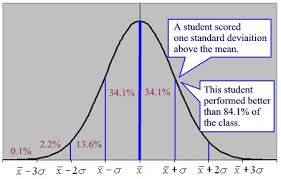
\includegraphics[width=\textwidth]{student_score}
  \end{center}
\end{minipage}

%\begin{minipage}{0.35\textwidth}
Men mag hier echter niet uit besluiten dat alles normaal verdeeld zou zijn. Typische voorbeelden van niet-normaal verdeelde gegevens zijn:

\begin{itemize}
  \item winst of verlies bij beursgang
  \item leeftijd bij het overlijden van mens of dier
  \item inkomen
\end{itemize}
%\end{minipage}
%\begin{minipage}{0.65\textwidth}
  \begin{center}
    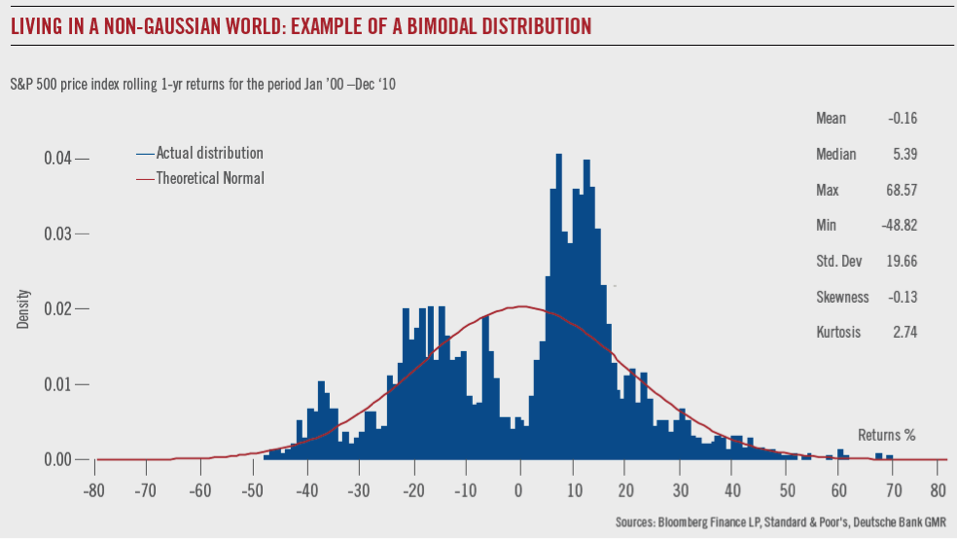
\includegraphics[width=\textwidth]{non-normal}
  \end{center}
%\end{minipage}

\pagebreak
\subsection{Definitie}

\begin{mdframed}
Een kansvariabele $X$ is {\bf normaal verdeeld} als haar kansfunctie $f$ gegeven wordt door
$$f(x)=\dfrac{1}{\sigma{\sqrt{2\pi}}}\;e^{-\dfrac{1}{2}\left(\dfrac{x-\mu}{\sigma}\right)^2}$$
\end{mdframed}

\paragraph*{Notatie}
Een kansvariabele $X$ die normaal verdeeld is wordt kort genoteerd met
$$X\sim N(\mu, \sigma)$$

Het is duidelijk dat de kansfunctie afhangt van twee parameters, het gemiddelde $\mu$ en de standaardafwijking $\sigma$ die de ligging van de verdeling bepalen.

\paragraph*{Eigenschappen van de normale verdeling}
\begin{mdframed}
Als $X\sim N(\mu, \sigma)$, dan geldt
\begin{itemize}
  \item verwachtingswaarde: $E(X)=\mu$
  \item variantie: $\Var(X)=\sigma^2$
  \item standaardafwijking: $\sigma$
\end{itemize}
\end{mdframed}

\subsection{Grafische betekenis van $\mu$ en $\sigma$}

\subsection*{Grafische betekenis van $\mu$}

We laten in het functievoorschrift van de normale verdeling
$$f(x)=\dfrac{1}{\sigma{\sqrt{2\pi}}}\;e^{-\dfrac{1}{2}\left(\dfrac{x-\mu}{\sigma}\right)^2}$$
het gemiddelde $\mu$ variëren, terwijl we de standaardafwijking $\sigma$ constant houden ($\sigma=1$). Hieronder zie je de grafieken voor verschillende waarden van $\mu$:
\begin{center}
\definecolor{cqcqcq}{rgb}{0.75,0.75,0.75}
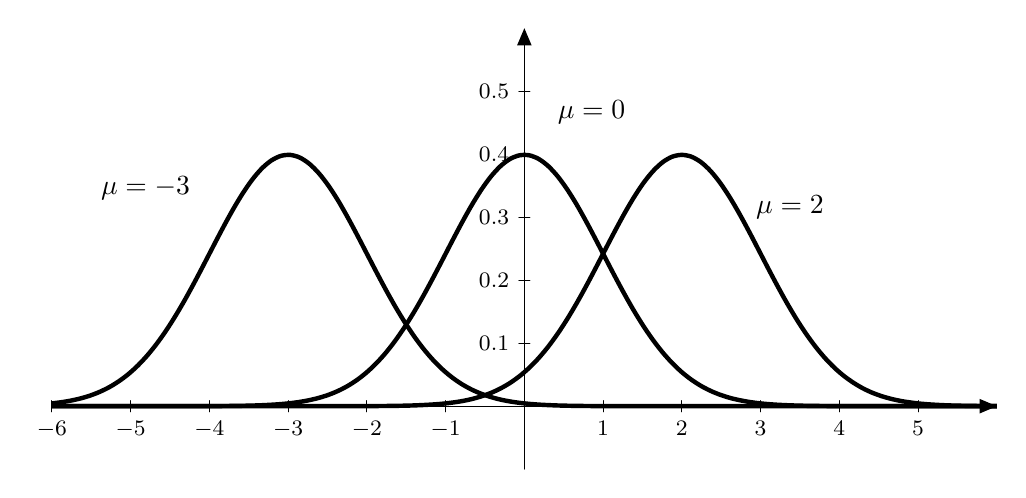
\begin{tikzpicture}[line cap=round,line join=round,>=triangle 45,x=1.0cm,y=8.0cm]
%\draw [color=cqcqcq,dash pattern=on 1pt off 1pt, xstep=1.0cm,ystep=1.0cm] (-6,-0.1) grid (6,0.6);
\draw[->,color=black] (-6,0) -- (6,0);
\foreach \x in {-6,-5,-4,-3,-2,-1,1,2,3,4,5}
\draw[shift={(\x,0)},color=black] (0pt,2pt) -- (0pt,-2pt) node[below] {\footnotesize $\x$};
\draw[->,color=black] (0,-0.1) -- (0,0.6);
\clip(-6,-0.1) rectangle (6,0.6);
\foreach \y in {,0.1,0.2,0.3,0.4,0.5}
\draw[shift={(0,\y)},color=black] (2pt,0pt) -- (-2pt,0pt) node[left] {\footnotesize $\y$};
\draw[line width=1.6pt, smooth,samples=100,domain=-6.0:6.0] plot(\x,{exp((-((\x))^2)/2)/(sqrt(2*3.1415926535)*abs(1))});
\draw[line width=1.6pt, smooth,samples=100,domain=-6.0:6.0] plot(\x,{exp((-((\x)+3)^2)/2)/(sqrt(2*3.1415926535)*abs(1))});
\draw[line width=1.6pt, smooth,samples=100,domain=-6.0:6.0] plot(\x,{exp((-((\x)-2)^2)/2)/(sqrt(2*3.1415926535)*abs(1))});
\draw (-5.5,0.38) node[anchor=north west] {$\mu=-3$};
\draw (0.3,0.5) node[anchor=north west] {$\mu=0$};
\draw (2.82,0.35) node[anchor=north west] {$\mu=2$};
\end{tikzpicture}
\end{center}

We merken dat de grafieken van al deze normale verdelingen met constante $\sigma=1$ op een verschuiving evenwijdig met de $x$-as met $\mu$ eenheden na gelijk zijn.

\begin{oefening}
Voor welke $x$-waarde vinden we steeds de top van de klokvormige kromme?
\end{oefening}

\subsection*{Grafische betekenis van $\sigma$}

We laten nu in het functievoorschrift
$$f(x)=\dfrac{1}{\sigma{\sqrt{2\pi}}}\;e^{-\dfrac{1}{2}\left(\dfrac{x-\mu}{\sigma}\right)^2}$$
de standaardafwijking $\sigma$ variëren, terwijl we het gemiddelde $\mu$ constant houden op $\mu=0$.

\begin{center}
\definecolor{cqcqcq}{rgb}{0.75,0.75,0.75}
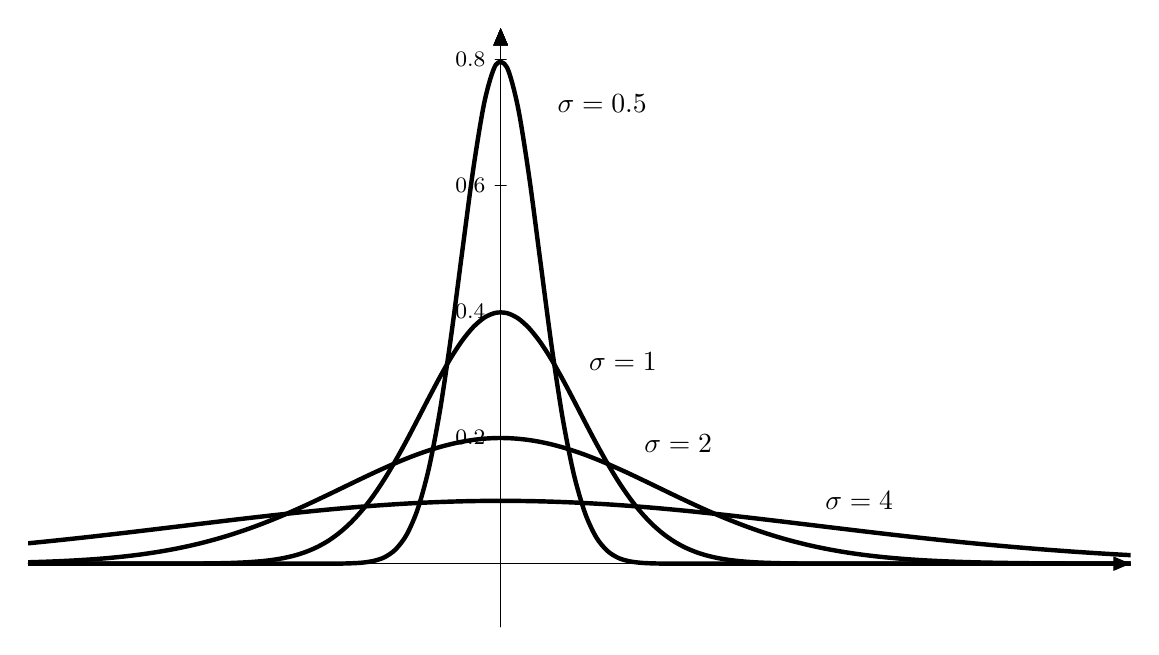
\begin{tikzpicture}[line cap=round,line join=round,>=triangle 45,x=1.0cm,y=8.0cm]
%\draw [color=cqcqcq,dash pattern=on 1pt off 1pt, xstep=2.0cm,ystep=0.2cm] (-5.5,-0.1) grid (5.5,0.85);
\draw[->,color=black] (-6,0) -- (8,0);
\foreach \x in {-6,-4,-2,2,4,6}
%\draw[shift={(\x,0)},color=black] (0pt,2pt) -- (0pt,-2pt) node[below] {\footnotesize $\x$};
\draw[->,color=black] (0,-0.1) -- (0,0.85);
\foreach \y in {0.2,0.4,0.6,0.8}
\draw[shift={(0,\y)},color=black] (2pt,0pt) -- (-2pt,0pt) node[left] {\footnotesize $\y$};
\clip(-6,-0.1) rectangle (8,0.85);
\draw[line width=1.6pt, smooth,samples=100,domain=-6.0:8.0] plot(\x,{exp((-((\x))^2)/2)/(sqrt(2*3.1415926535)*abs(1))});
\draw[line width=1.6pt, smooth,samples=100,domain=-6.0:8.0] plot(\x,{exp((-(((\x))/0.5)^2)/2)/(sqrt(2*3.1415926535)*abs(0.5))});
\draw[line width=1.6pt, smooth,samples=100,domain=-6.0:8.0] plot(\x,{exp((-(((\x))/2)^2)/2)/(sqrt(2*3.1415926535)*abs(2))});
\draw[line width=1.6pt, smooth,samples=100,domain=-6.0:8.0] plot(\x,{exp((-(((\x))/4)^2)/2)/(sqrt(2*3.1415926535)*abs(4))});
\draw (0.6,0.76) node[anchor=north west] {$\sigma=0.5$};
\draw (1.0,0.35) node[anchor=north west] {$\sigma=1$};
\draw (1.7,0.22) node[anchor=north west] {$\sigma=2$};
\draw (4,0.13) node[anchor=north west] {$\sigma=4$};
\end{tikzpicture}
\end{center}

We merken dat de grafieken van al deze normale verdelingen met constante $\mu=0$ qua vorm gelijk zijn. Ze hebben wel allemaal een uitrekking of inkrimping evenwijdig met de $y$-as ondergaan.

\begin{oefening}
Vul volgende tabel aan:
\begin{center}
  \begin{tabular}{c|c}
    $\sigma$ & Hoogte van de top\\
    \hline
    0.5 & \arule{2cm}\\
    1 & \arule{2cm}\\
    2 & \arule{2cm}\\
    4 & \arule{2cm}\\
    \vdots & \vdots\\
    $\sigma$ & \arule{2cm}
  \end{tabular}
\end{center}
\end{oefening}

\paragraph*{Besluit grafische betekenis van $\mu$ en $\sigma$}
\begin{mdframed}
Voor elke $x$ geldt $f(\mu-x)=f(\mu+x)$. $f$ is dus {\em symmetrisch} ten opzichte van $x=\mu$. In $\mu$ bereikt $f$ haar {\em maximum}. De waarde van $\mu$ bepaalt dus de centrale ligging en de waarde van $\sigma$ bepaalt de spreiding. Aan de hand van de spreiding vinden we ook de hoogte van de top, namelijk $\frac{0.4}{\sigma}$.
\end{mdframed}

\begin{oefening}
Bepaal in de onderstaande grafieken het gemiddelde $\mu$ en de standaardafwijking $\sigma$ van de vet gedrukte functie.

\definecolor{cqcqcq}{rgb}{0.75,0.75,0.75}
\begin{multicols}{2}
\begin{center}
\begin{tikzpicture}[xscale=0.6,yscale=5,line cap=round,line join=round,>=triangle 45,x=1.0cm,y=1.0cm]
\draw [color=cqcqcq,dash pattern=on 1pt off 1pt, xstep=2.0cm,ystep=0.2cm] (-5.9,-0.1) grid (5.9,0.9);
\draw[->,color=black] (-6,0) -- (6,0);
\foreach \x in {-4,-2,2,4}
\draw[shift={(\x,0)},color=black] (0pt,2pt) -- (0pt,-2pt) node[below] {\footnotesize $\x$};
\draw[->,color=black] (0,-0.1) -- (0,1);
\foreach \y in {,0.2,0.4,0.6,0.8}
\draw[shift={(0,\y)},color=black] (2pt,0pt) -- (-2pt,0pt) node[left] {\footnotesize $\y$};
\clip(-6,-0.1) rectangle (6,1);
\draw[line width=1.2pt, smooth,samples=100,domain=-6.0:6.0] plot(\x,{exp((-((\x))^2)/2)/(sqrt(2*3.1415926535)*abs(1))});
\draw[line width=2pt, smooth,samples=100,domain=-6.0:6.0] plot(\x,{exp((-(((\x)-3)/0.5)^2)/2)/(sqrt(2*3.1415926535)*abs(0.5))});
\end{tikzpicture}
$$\mu=\arule{1cm} \sigma=\arule{1cm}$$
\end{center}

\begin{center}
\begin{tikzpicture}[xscale=0.6,yscale=5,line cap=round,line join=round,>=triangle 45,x=1.0cm,y=1.0cm]
\draw [color=cqcqcq,dash pattern=on 1pt off 1pt, xstep=2.0cm,ystep=0.2cm] (-5.9,-0.1) grid (5.9,0.9);
\draw[->,color=black] (-6,0) -- (6,0);
\foreach \x in {-4,-2,2,4}
\draw[shift={(\x,0)},color=black] (0pt,2pt) -- (0pt,-2pt) node[below] {\footnotesize $\x$};
\draw[->,color=black] (0,-0.1) -- (0,1);
\foreach \y in {,0.2,0.4,0.6,0.8}
\draw[shift={(0,\y)},color=black] (2pt,0pt) -- (-2pt,0pt) node[left] {\footnotesize $\y$};
\clip(-6,-0.1) rectangle (6,1);
\draw[line width=1.2pt, smooth,samples=100,domain=-6.0:6.0] plot(\x,{exp((-((\x))^2)/2)/(sqrt(2*3.1415926535)*abs(1))});
\draw[line width=2pt, smooth,samples=100,domain=-6.0:6.0] plot(\x,{exp((-(((\x)+2)/2)^2)/2)/(sqrt(2*3.1415926535)*abs(2))});
\end{tikzpicture}
$$\mu=\arule{1cm} \sigma=\arule{1cm}$$
\end{center}

\begin{center}
\begin{tikzpicture}[xscale=0.6,yscale=5,line cap=round,line join=round,>=triangle 45,x=1.0cm,y=1.0cm]
\draw [color=cqcqcq,dash pattern=on 1pt off 1pt, xstep=2.0cm,ystep=0.2cm] (-5.9,-0.1) grid (5.9,0.9);
\draw[->,color=black] (-6,0) -- (6,0);
\foreach \x in {-4,-2,2,4}
\draw[shift={(\x,0)},color=black] (0pt,2pt) -- (0pt,-2pt) node[below] {\footnotesize $\x$};
\draw[->,color=black] (0,-0.1) -- (0,1);
\foreach \y in {,0.2,0.4,0.6,0.8}
\draw[shift={(0,\y)},color=black] (2pt,0pt) -- (-2pt,0pt) node[left] {\footnotesize $\y$};
\clip(-6,-0.1) rectangle (6,1);
\draw[line width=1.2pt, smooth,samples=100,domain=-6.0:6.0] plot(\x,{exp((-((\x))^2)/2)/(sqrt(2*3.1415926535)*abs(1))});
\draw[line width=2pt, smooth,samples=100,domain=-6.0:6.0] plot(\x,{exp((-(((\x)+3)/1)^2)/2)/(sqrt(2*3.1415926535)*abs(1))});
\end{tikzpicture}
$$\mu=\arule{1cm} \sigma=\arule{1cm}$$
\end{center}

\begin{center}
\begin{tikzpicture}[xscale=0.6,yscale=5,line cap=round,line join=round,>=triangle 45,x=1.0cm,y=1.0cm]
\draw [color=cqcqcq,dash pattern=on 1pt off 1pt, xstep=2.0cm,ystep=0.2cm] (-5.9,-0.1) grid (5.9,0.9);
\draw[->,color=black] (-6,0) -- (6,0);
\foreach \x in {-4,-2,2,4}
\draw[shift={(\x,0)},color=black] (0pt,2pt) -- (0pt,-2pt) node[below] {\footnotesize $\x$};
\draw[->,color=black] (0,-0.1) -- (0,1);
\foreach \y in {,0.2,0.4,0.6,0.8}
\draw[shift={(0,\y)},color=black] (2pt,0pt) -- (-2pt,0pt) node[left] {\footnotesize $\y$};
\clip(-6,-0.1) rectangle (6,1);
\draw[line width=1.2pt, smooth,samples=100,domain=-6.0:6.0] plot(\x,{exp((-((\x))^2)/2)/(sqrt(2*3.1415926535)*abs(1))});
\draw[line width=2pt, smooth,samples=100,domain=-6.0:6.0] plot(\x,{exp((-(((\x)-0)/4)^2)/2)/(sqrt(2*3.1415926535)*abs(4))});
\end{tikzpicture}
$$\mu=\arule{1cm} \sigma=\arule{1cm}$$
\end{center}
\end{multicols}
\end{oefening}

\pagebreak
\section{Standaardnormale kansverdeling}

In de vorige paragraaf werden grafieken van de normale verdeling verschoven (met behulp van $\mu$) en herschaald (met behulp van $\sigma$). Het is dus mogelijk om de normale verdeling te
\begin{itemize}
  \item verschuiven zodat het gemiddelde $\mu=0$ wordt,
  \item herschalen zodat de standaardafwijking $\sigma=1$ wordt.
\end{itemize}

Een normale verdelingen met gemiddelde 0 en standaardafwijking 1 of kort $N(0,1)$ noemen we {\bf standaardnormaal verdeeld}. Om aan te duiden dat we met de standaardnormale verdeling werken, gebruiken we de letter $Z$ i.p.v. $X$ om de kansvariabele aan te duiden.

Een normale verdeling herken je aan de grafiek van de kansfunctie. De grafiek is namelijk steeds een symmetrische, ééntoppige, klokvormige kromme. Op de volgende figuur zie je de grafiek horend bij N(0, 1).

\begin{center}
\begin{tikzpicture}
\begin{axis}[
  no markers, domain=0:10, samples=100,
  axis lines*=left, xlabel=$x$, ylabel=$f(x)$,
  every axis y label/.style={at={(0,1)},anchor=south},
  every axis x label/.style={at=(current axis.right of origin),anchor=west},
  height=8cm, width=16cm,
  xtick={-3,-2,-1,0,1,2,3}, ytick={0.1, 0.2, 0.3, 0.4},
  enlargelimits=false, clip=false, axis on top,
  grid = none
  ]
  \addplot [fill=gray!40, draw=none, domain=-1:1] {gauss(0,1)} \closedcycle;
  \addplot [very thick,black!50!black, domain=-4:4] {gauss(0,1)};
  \draw [yshift=-0.6cm] (axis cs:0,0) node[anchor=north] {$\mu$};
  \draw [yshift=-0.6cm] (axis cs:-1,0) node[anchor=north] {$-\sigma$};
  \draw [yshift=-0.6cm] (axis cs:1,0) node[anchor=north] {$\sigma$};
  \draw (axis cs:0,0.2) node[anchor=north] {$\pm 68.27\%$};
\end{axis}
\end{tikzpicture}
\end{center}

Voor de standaardnormale verdeling $N(0,1)$ worden de verdelingsfunctie $F(x)$, verwachtingswaarde $E(X)$ en standaardafwijking $\sigma$ gegeven door
\begin{itemize}
  \item $F(z)=P(Z\leq z)=\Phi(z)$ (zie verder)
  \item $E(Z)=\mu=0$
  \item $\sigma=1$
\end{itemize}

\subsection{Kansen berekenen bij standaardnormaal verdeelde populaties}

Om de kans te berekenen dat iemand minder heeft dan een bepaalde waarde, volstaat het om de oppervlakte onder de kromme te berekenen, zoals in onderstaande figuur:

\begin{center}
\begin{tikzpicture}
\begin{axis}[
  no markers, domain=0:10, samples=100,
  axis lines*=left, xlabel=$x$, ylabel=$f(x)$,
  every axis y label/.style={at={(0,1)},anchor=south},
  every axis x label/.style={at=(current axis.right of origin),anchor=west},
  height=8cm, width=16cm,
  xtick={0,1}, ytick={0.1, 0.2, 0.3, 0.4},
  enlargelimits=false, clip=false, axis on top,
  grid = none
  ]
  \addplot [fill=gray!40, draw=none, domain=-4:1.5] {gauss(0,1)} \closedcycle;
  \addplot [very thick,black!50!black, domain=-4:4] {gauss(0,1)};
  \draw [yshift=-0.1cm] (axis cs:1.5,0) node[anchor=north] {$z$};
  \draw (axis cs:0,0.2) node[anchor=north] {$\Phi(z)$};
\end{axis}
\end{tikzpicture}
\end{center}

De leerlingen die ook integraalrekenen krijgen zien onmiddellijk dat dit niets anders is dan de integraal
$$\Phi(z)=P(Z\leq z)=\dfrac{1}{\sqrt{2\pi}}\int_{-\infty}^{z}e^{-\frac{1}{2}t^2}dt\;.$$

Het berekenen van deze oppervlakteintegraal is vrij ingewikkeld. Voor de standaardnormale verdeling bestaat er echter een tabel waaruit je deze kansen rechtstreeks kan aflezen, zie bijlage.

\subsubsection*{Voorbeeld 1}

Gegeven: Een populatie die kan beschreven worden door een standaardnormale verdeling. Bereken het percentage waarnemingen kleiner dan $1.36$.

In symbolen: $\Phi(1.36)=P(Z\leq 1.36)$

Methode:
\begin{itemize}
  \item Zoek de waarde $1.36$ in de tabel.
  \begin{itemize}
    \item Voor de eerste 2 cijfers kijk je in de linkerkolom van de tabel: ga op zoek naar de rij die overeenstemt met de waarde 1.3.
    \item Vervolgens schuif je op naar rechts tot de kolom die overeenkomt met 0.06.
  \end{itemize}
  \item Het percentage waarnemingen kleiner dan 1.36 bedraagt dus 91.308\%
\end{itemize}

\begin{minipage}{0.5\textwidth}
$$\Phi(1.36)=P(Z\leq 1.36)=0.91308$$
$$\Rightarrow\Phi(1.36)=91.308\%$$
\end{minipage}
\begin{minipage}{0.5\textwidth}
\vspace*{0.8cm}
\begin{center}
\begin{tikzpicture}
\begin{axis}[
  no markers, domain=0:10, samples=100,
  axis lines*=left,
  height=4cm, width=8cm,
  xtick={1.36}, ytick={0}, yticklabels={},
  enlargelimits=false, clip=false, axis on top,
  grid = none
  ]
  \addplot [fill=gray!40, draw=none, domain=-4:1.36] {gauss(0,1)} \closedcycle;
  \addplot [very thick,black!50!black, domain=-4:4] {gauss(0,1)};
  \draw (axis cs:0,0.2) node[anchor=north] {$91\%$};
\end{axis}
\end{tikzpicture}
\end{center}
\end{minipage}

\subsubsection*{Voorbeeld 2}

Gegeven: Een populatie die kan beschreven worden door een standaardnormale verdeling. Bereken het percentage waarnemingen gelegen tussen $1.03$ en $2.95$.

In symbolen: $P(1.03\leq Z\leq 2.95)$

Dit is niet rechtstreeks in de tabel af te lezen. We herschrijven het gevraagde als volgt (zie figuur ter verduidelijking):

\begin{align*}
  P(1.03\leq Z\leq 2.95) &= P(Z\leq 2.95) - P(Z\leq 1.03)\\
                         &= \Phi(2.95) - \Phi(1.03)
\end{align*}

\begin{center}
\begin{tikzpicture}
\begin{axis}[
  no markers, domain=0:10, samples=100,
  axis lines*=left,
  height=6cm, width=14cm,
  xtick={1.03, 2.95}, ytick={0}, yticklabels={},
  enlargelimits=false, clip=false, axis on top,
  grid = none
  ]
  \addplot [fill=gray!40, draw=none, domain=1.03:2.95] {gauss(0,1)} \closedcycle;
  \addplot [very thick,black!50!black, domain=-4:4] {gauss(0,1)};
  %\draw (axis cs:0,0.2) node[anchor=north] {$91\%$};
\end{axis}
\end{tikzpicture}
\end{center}

\subsubsection*{Voorbeeld 3}

Gegeven: Een populatie die kan beschreven worden door een standaardnormale verdeling. Bereken het percentage waarnemingen kleiner dan $-2.07$.

In symbolen: $P(Z\leq -2.07)$

Ook dit is niet rechtstreeks uit de tabel af te lezen, maar we kunnen het gevraagde opnieuw herschrijven tot iets dat wel uit de tabel af te lezen is:

\begin{minipage}{0.5\textwidth}
\begin{align*}
  P(Z\leq -2.07) &= P(Z \geq 2.07)\\
                 &= 1 - P(Z \leq 2.07)\\
                 &= 1 - \Phi(2.07)
\end{align*}
\end{minipage}
\begin{minipage}{0.5\textwidth}
\vspace*{1cm}
\begin{center}
\begin{tikzpicture}
\begin{axis}[
  no markers, domain=0:10, samples=100,
  axis lines*=left,
  height=4cm, width=10cm,
  xtick={-2.07}, ytick={0}, yticklabels={},
  enlargelimits=false, clip=false, axis on top,
  grid = none
  ]
  \addplot [fill=gray!40, draw=none, domain=-4:-2.07] {gauss(0,1)} \closedcycle;
  \addplot [very thick,black!50!black, domain=-4:4] {gauss(0,1)};
  %\draw (axis cs:0,0.2) node[anchor=north] {$91\%$};
\end{axis}
\end{tikzpicture}
\end{center}
\end{minipage}

\pagebreak
\subsection{Overzicht formules}
\begin{multicols}{2}
  $$P(Z\leq a)=\Phi(a)$$
  $$P(Z\geq a)=1-\Phi(a)$$
  $$P(Z\leq -a)=1-\Phi(a)$$
  $$P(Z\geq -a)=\Phi(a)$$
  \vfill
  $$P(a\leq Z \leq b)=\Phi(b)-\Phi(a)$$
  $$P(-a\leq Z \leq b)=\Phi(b)+\Phi(a)-1$$
  $$P(-a\leq Z \leq -b)=\Phi(a)-\Phi(b)$$
\end{multicols}

Het is niet nodig om deze formules uit het hoofd te leren. Maak een schets van de standaardnormale en duid er het gevraagde gebied op aan. Beredeneer dan zelf hoe je aan het gebied komt door enkel $\Phi(z)$ te gebruiken.

\subsection{Oefeningen}

\begin{oefening}
Bepaal met de tabel van de standaardnormale verdeling volgende kansen, maak telkens een verduidelijkende schets:
\begin{enumerate}[(a)]
  \item $P(Z\leq 0.97)$
  \item $P(Z\leq 0.71)$
  \item $P(2\leq Z \leq 2.5)$
  \item $P(Z \leq -0.44)$
  \item $P(1.42 \leq Z \leq 2.42)$
\end{enumerate}
\end{oefening}

\begin{oefening}
Bepaal volgende kansen, {\bf zonder} gebruik te maken van de tabel van de standaardnormale:
\begin{enumerate}[(a)]
  \item $P(-\infty\leq Z \leq +\infty)$
  \item $P(Z\leq 0)$
  \item $P(Z\geq 0)$
\end{enumerate}
\end{oefening}


\pagebreak
\section{Kansen berekenen bij de normale verdeling}

\subsection{Standaardisering}

We hebben gezien dat alle normale verdelingen dezelfde vorm hebben, op een horizontale verschuiving of verticale uitrekking na. De kansdichtheidsfunctie van een normale verdeling kan dus steeds
\begin{itemize}
  \item verschoven worden zodat het gemiddelde $\mu=0$ wordt,
  \item herschaald worden zodat de standaardafwijking $\sigma=1$ wordt.
\end{itemize}

Dit wil zeggen dat een kansvariabele die een normale verdeling volgt steeds {\em gestandaardiseerd} kan worden tot een andere kansvariabele die eveneens normaal verdeeld is, maar met gemiddelde 0 en standaardafwijking 1

\subsection{Z-Score}

Om een waarneming $x$ te standaardiseren wordt het gemiddelde ervan afgetrokken en vervolgens gedeeld door de standaardafwijking $\sigma$. We noteren deze {\em gestandaardiseerde waarde} van $x$ de $z$-score en noteren ze met de letter $z$. Dus
$z=\dfrac{x-\mu}{\sigma}\;.$

\paragraph*{Gestandaardiseerde normale verdeling}
\begin{mdframed}
Als $X$ een kansvariabele is met $X\sim N(\mu,\sigma)$, dan volgt de kansvariabele $Z$ gegeven door
$$Z=\dfrac{X-\mu}{\sigma}$$
de standaardnormale verdeling. Er geldt dus $Z\sim N(0,1)$.
\end{mdframed}

Een $z$-score geeft aan hoeveel standaardafwijkingen de oorspronkelijke waarneming van het gemiddelde verwijderd is en in welke richting. Waarnemingen groter dan het gemiddelde geven een positieve $z$-score, waarnemingen die kleiner zijn dan het gemiddelde een negatieve.

$z$-scores worden o.a. gebruikt om waarnemingen uit verschillende populaties en/of steekproeven met elkaar te vergelijken.

\begin{oefening}
Robbe zit in klas A en behaalde op zijn laatste toets wiskunde 14 op 20. Het klasgemiddelde was 11 met een standaardafwijking van 3.\\
Zijn zus Kathy zit in klas B en behaalde op haar laatste toets wiskunde 23 op 30. Het klasgemiddelde was 19 met een standaardafwijking van 5.\\
Wie heeft nu relatief gezien het beste gewerkt?
\end{oefening}

\subsection{Kansen berekenen}

Omdat er geen tabellen bestaan voor de niet-standaard normaal verdeelde populaties, herleiden we de normaal verdeelde waarnemingen tot standaardnormaal verdeelde waarnemingen met behulp van de $z$-score.

\subsubsection*{Voorbeeld}

\underline{Gegeven:} Een normaal verdeelde populatie met gemiddelde $\mu=20$ en standaardafwijking $\sigma=4$. Bereken het percentage waarnemingen kleiner dan 22.\\
\underline{Methode:}
\begin{enumerate}[(a)]
  \item We berekenen eerst de $z$-score van $x=22$:
  $$z=\dfrac{x-\mu}{\sigma}=\dfrac{22-20}{4}=0.5$$
  \item Vervolgens zoeken we in de tabel van de standaardnormale verdeling het percentage waarnemingen met een $z$-score kleiner dan $0.5$:
  $$P(X\leq 22)=P(Z\leq 0.5)=\Phi(0.5)=0.69146=69.15\%$$
  \item Antwoord: $30.85\%$ van de waarnemingen is kleiner dan $22$.
\end{enumerate}

\paragraph*{Opmerking: } De $z$-score mag afgerond worden op $2$ cijfers na de komma want de tabel achteraan is maar correct op 2 cijfers na de komma.

\begin{oefening}
Het gewicht van een bepaalde soort peer is bij benadering normaal verdeeld met gemiddelde 150g en standaardafwijking 30g.
Welke percentage peren weegt minder dan 125g?
\begin{enumerate}[(a)]
  \item Bereken eerst de $z$-score van $x=125$.
  \arules{2}
  \item Bepaal nu met behulp van de tabel de kans dat een peer minder weegt dan $125\g$.
  \arules{4}
  \item Formuleer nu je antwoord.
  \arules{1}
\end{enumerate}
\end{oefening}

\subsection{Oefeningen}

\begin{oefening}
De voetlengten van volwassen vrouwen zijn bij benadering normaal verdeeld met een gemiddelde van $26.3 \cm$ en een standaardafwijking van $2.7 \cm$.
\begin{enumerate}[(a)]
  \item Welk percentage heeft een voetlengte die kleiner is dan $25 \cm$?
  \item Welk percentage heeft een voetlengte die groter is dan $28 \cm$?
\end{enumerate}
\end{oefening}

\begin{oefening}
De tijd die huisarts A tijdens zijn spreekuur aan een patiënt besteedt, is bij benadering normaal verdeeld met een gemiddelde van 15 minuten en een standaardafwijking van 3.4 minuten.
\begin{enumerate}[(a)]
  \item Welk percentage van de patiënten valt in de categorie van consultaties die beneden de 10 minuten valt?
  \item Welk percentage van de consultatie duurt tussen 14 en 18 minuten?
  \item Welk percentage van de consultaties duurt langer dan 18 minuten?
\end{enumerate}
\end{oefening}

\begin{oefening}
Vaak worden in de statistiek gerekend met ‘mooie’ betrouwbaarheidsintervallen, zoals 90\%, 95\% en 99\%. Bepaal bij elk percentage de bijhorende $z$-score.
\end{oefening}

\begin{oefening}
Welk van de volgende resultaten op een examen statistiek is het meest uitzonderlijke?
\begin{enumerate}[(A)]
  \item 16 in een groep met gemiddelde 15 en standaardafwijking 1.27
  \item 17 in een groep met gemiddelde 16 en standaardafwijking 2.45
  \item 16 in een groep met gemiddelde 13 en standaardafwijking 0.50
  \item 17 in een groep met gemiddelde 17 en standaardafwijking 0.12
  \item 16 in een groep met gemiddelde 15 en standaardafwijking 3
\end{enumerate}
\end{oefening}

\begin{oefening}
Punten van verschillende leerlingen in eenzelfde klas zouden normaal verdeeld moeten zijn. We kunnen dit gebruiken om {\em relatief gezien} je beste resultaat over de verschillende dagelijkse werken te vinden. Maak hiervoor een tabel met 5 kolommen als volgt:
\begin{center}
  \begin{tabular}{l|c|c|c|c}
  Leerling & DW2 & Z-score DW2 & DW3 & Z-score DW3\\
  \hline
  \vdots&&&&\\
%  \vdots&&&&\\
%  \vdots&&&&\\
  \hline
  gemiddelde&&&&\\
  standaardafwijking&&&&\\
  \end{tabular}
\end{center}
Je kan dit bijvoorbeeld gebruiken wanneer je absoluut gezien een lager cijfer hebt bij DW3, maar relatief gezien een hoger cijfer bij DW3 om je ouders gerust te stellen.
\end{oefening}

\pagebreak
\section{Binomiale verdeling benaderen door een normale verdeling}

\begin{oefening}
Vroeger moest men aan de universiteit een 12 op 20 halen voor een vak om zeker geslaagd te zijn in eerste zit voor dat vak. Want haalde je voor één van de andere vakken minder dan 10 op 20, dan moest je een herexamen doen voor alle vakken onder de 12.\\
Bereken de kans om minstens 60\% te halen op een meerkeuze examens bestaande uit 50 vragen met telkens 4 keuzes en zonder gok correctie, die je volledig willekeurig beantwoordt?
\end{oefening}

Leerlingen die de vorige oefening wensen te maken zullen snel inzien dat het hier een binomiale verdeling
$$X\sim B(50, 1/4)$$
betreft en dat ze minimaal 30 keer de formule
$$f(k)=C_{50}^{k}(1/4)^k(3/4)^{n-k}$$
moeten gebruiken om $P(X\geq 30)=f(30)+f(31)+\cdots +f(50)$ uit te rekenen. Laten we in de plaats van het vele rekenen eens kijken naar de grafiek van de kansfunctie met behulp van {\em Geogebra}. Als we in het invoervenster het commando \verb#BinomialDist[50,1/4]# ingeven krijgen we de volgende plot:

\begin{center}
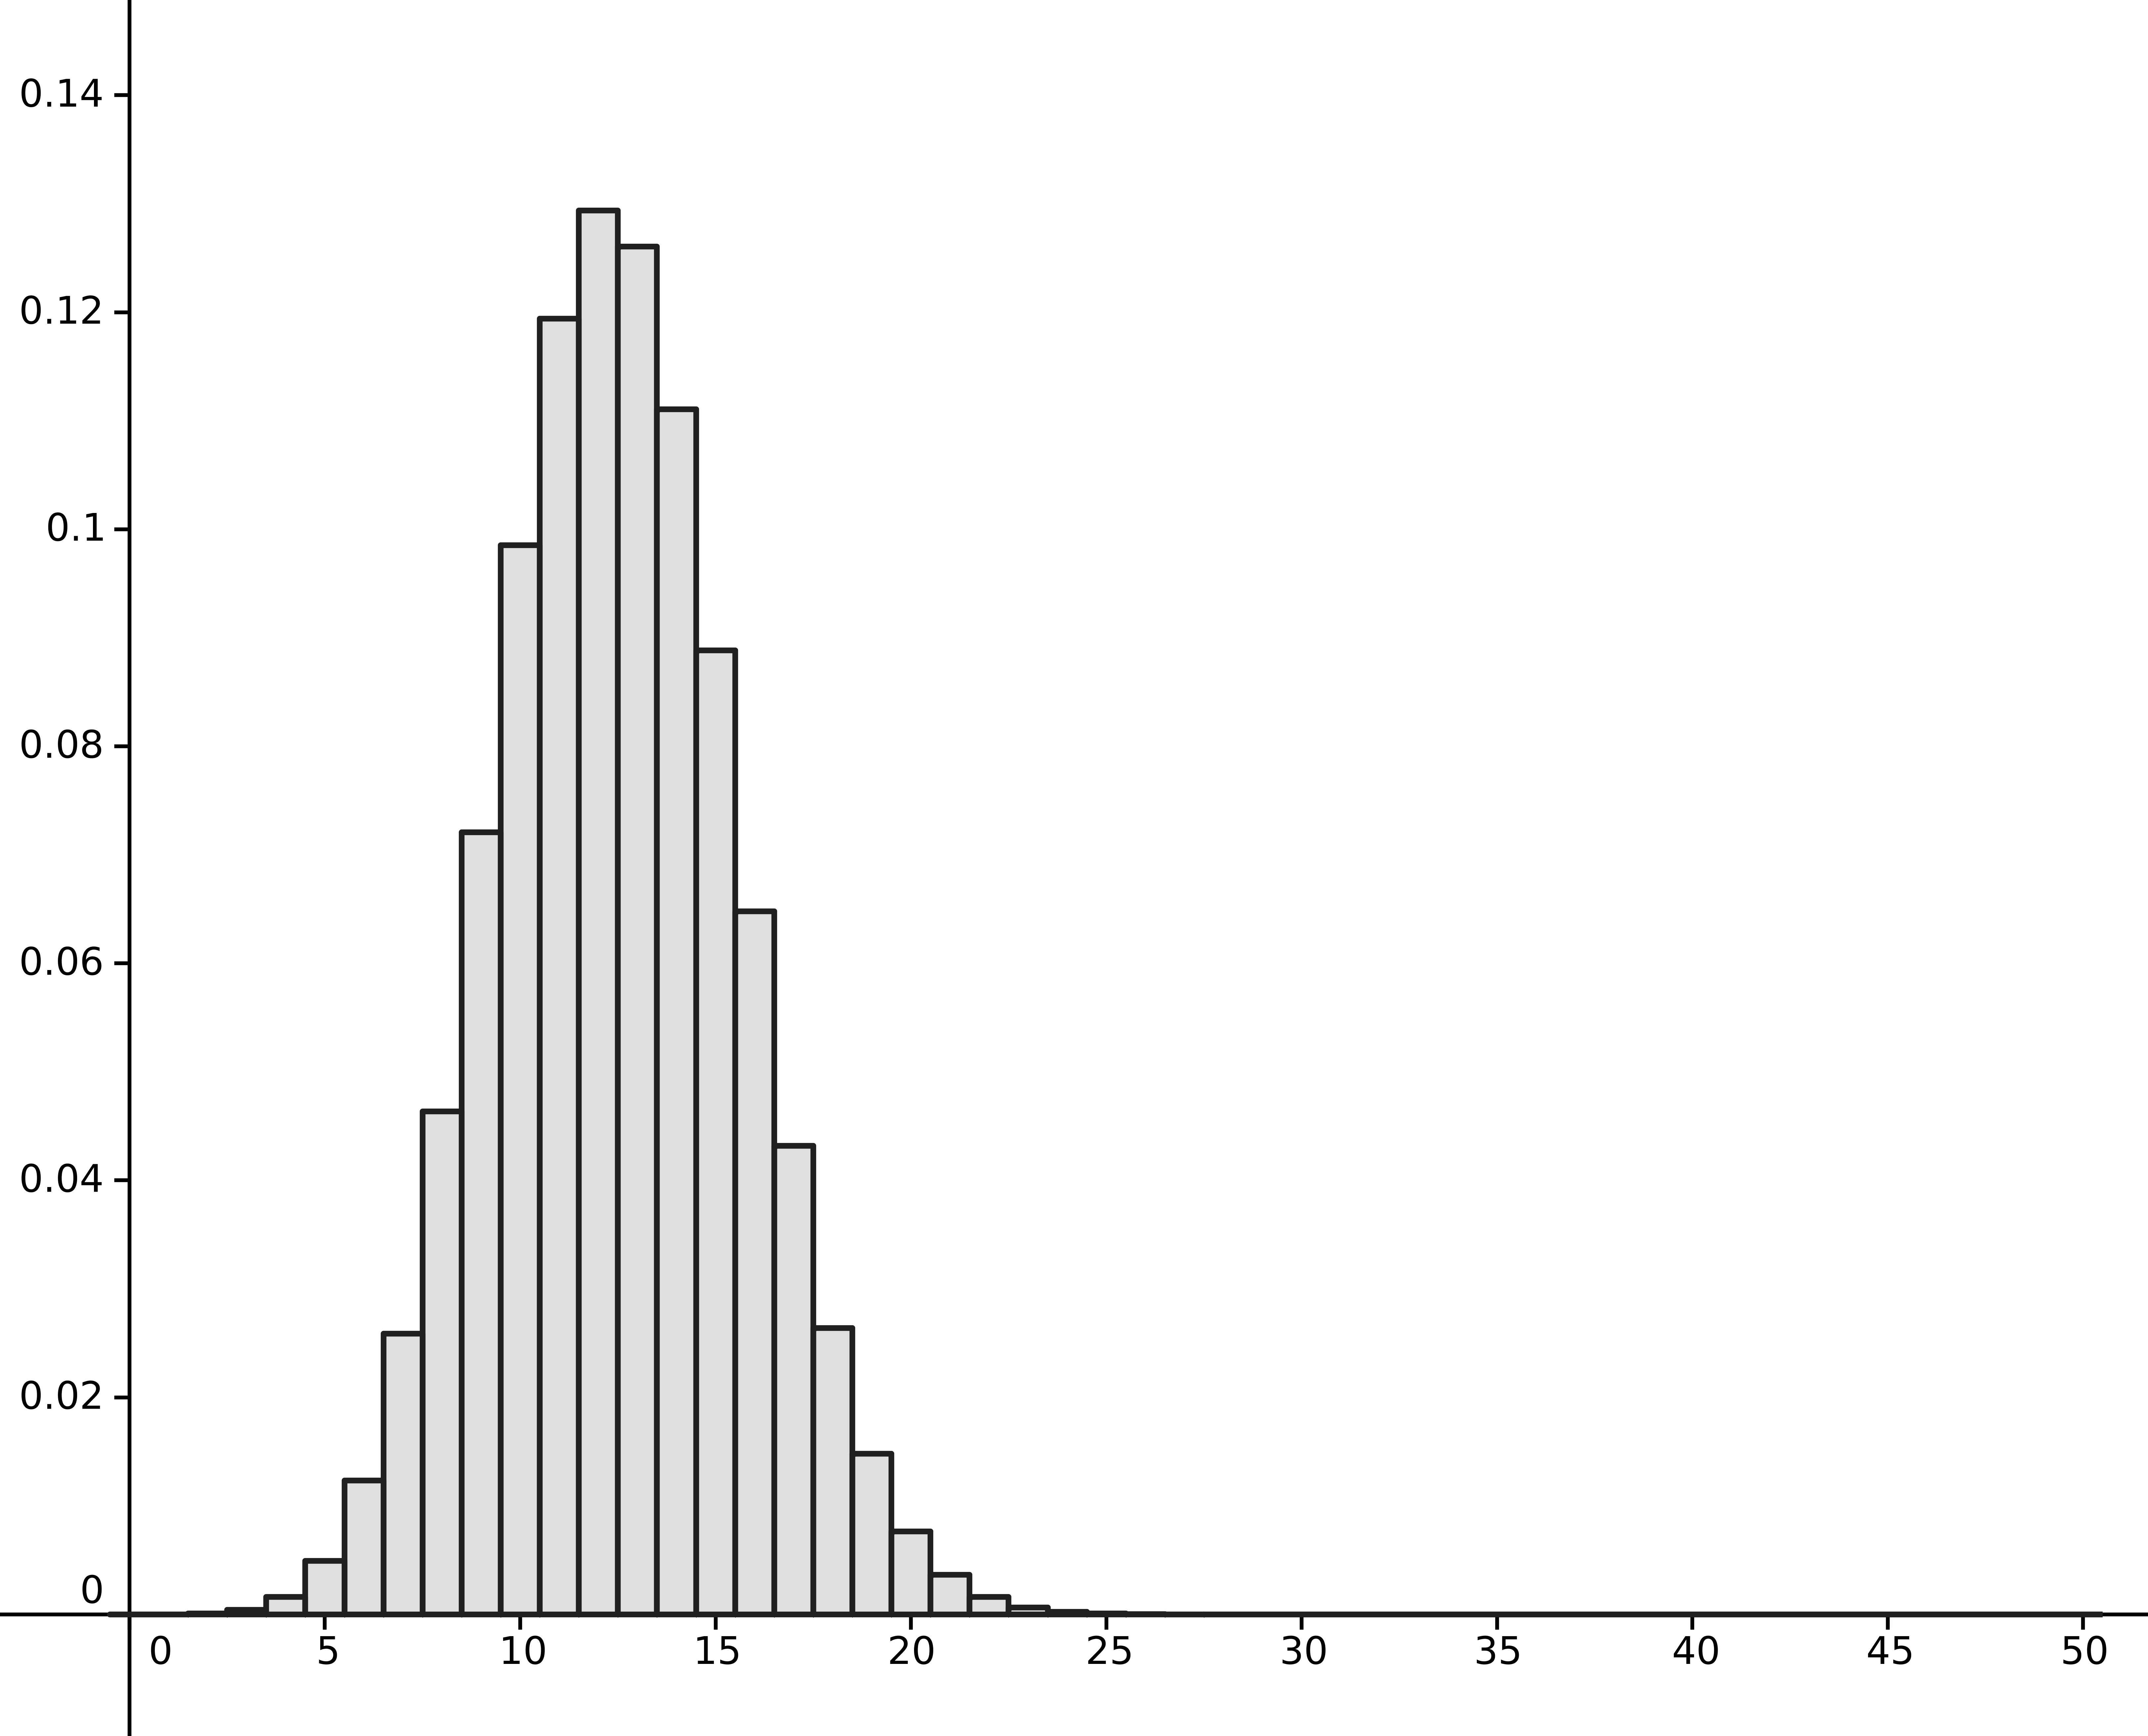
\includegraphics[width=0.7\textwidth]{binomial_punten}
\end{center}

Merk op dat we de $x$ waarden door hebben laten lopen tot aan $x=50$ want de kans is niet onbestaand dat we heel veel geluk hebben en dat we alle vragen juist beantwoorden.

\begin{oefening}
Bereken voor voorgaande oefening de verwachtingswaarde, standaardafwijking en de hoogte van de top. Duid deze aan op de bovenstaande grafiek.
\begin{itemize}
  \item $\mu=E(X)=n\cdot p=$ \arulefill
  \item $\sigma=\sqrt{n\cdot p\cdot q}=$ \arulefill
  \item hoogte top: \arulefill
\end{itemize}
\end{oefening}

Mochten we nu de toppen van bovenstaande staafjes verbinden met een lijn, dan merken we op dat deze lijn goed te benaderen is door een normale verdeling met hetzelfde gemiddelde $\mu$ als de verwachtingswaarde en met dezelfde standaardafwijking $\sigma$ als die bij de binomiale verdeling horen.

Deze benadering zal steeds gelden voor voldoende grote $n$, we zullen afspreken

\paragraph*{Binomiale verdeling benaderen}
\begin{mdframed}
Een binomiale verdeling $X\sim B(n,p)$ met verwachtingswaarde $\mu$ en standaardafwijking $\sigma$ mag worden benaderd door een normale verdeling
$$B(n,p)\sim N(\mu,\sigma)$$
op voorwaarde dat $n\cdot p\geq5$, $n\cdot q\geq5$ en $n\geq 20$.
\end{mdframed}

\paragraph*{Opmerking} De binomiale verdeling is een discrete verdeling. Ze wordt nu dus benaderd door een continue verdeling.

Kansen berekenen van een binomiale verdeling wordt nu kinderspel, want de binomiale verdeling is normaal verdeeld en de normale verdeling kunnen we standaardiseren. We hoeven dus enkel maar nog op te zoeken in de tabel.

\begin{oefening}
Bereken de kans om minstens 60\% te halen op een meerkeuze examen bestaande uit 50 vragen
met telkens 4 keuzes en zonder gok correctie, die je volledig willekeurig beantwoordt?
\begin{enumerate}[(a)]
  \itemsep0.2em
  \item Bepaal de verdeling van de opgave: \arulefill
  \item Controleer de randvoorwaarden om te zien of we kunnen overgaan naar een normale verdeling:
  \arules{3}
  \item Ga over naar de normale verdeling: \arulefill
  \item Bereken de $z$-score:\arulefill
  \item Bepaal de gevraagde kans:
  \arules{1}
  \item Antwoord: \arulefill
\end{enumerate}
\end{oefening}

%\subsection{Oefeningen}

\begin{oefening}
Van een groot aantal schapen in een bepaald gebied is één op de twintig bruin. We willen de kans weten dat bij een steekproef van 1200 schapen het aantal bruine schapen niet groter dan 50 is.
\end{oefening}

\begin{oefening}
Ongeveer 1 op elke 20 mannen heeft last van "rood-groen" kleurenblindheid.
\begin{enumerate}[(a)]
  \item Hoe groot is de kans dat in een representatieve steekproef van 15.000 mannen juist 750 rood-groen-kleurenblinden voorkomen?
  \item Hoe groot is de kans dat in een representatieve steekproef van 15.000 mannen minstens 750 rood-groen-kleurenblinden voorkomen?
  \item Hoe groot is de kans dat in een representatieve steekproef van 15.000 mannen meer dan 750 rood-groen-kleurenblinden voorkomen?
\end{enumerate}
\end{oefening}

\begin{oefening}
De kans op kleurenblindheid is bij vrouwen veel kleiner, maar ongeveer 0.4\% van de Westerse vrouwen is kleurenblind.
Hoe groot is de kans dat in een representatieve steekproef van 250 vrouwen inderdaad 1 kleurenblinde voorkomt?
\end{oefening}

\begin{oefening}
Je gooit 15 keer met een eerlijk geldstuk. Het gaat je om de kans dat je hoogstens 6 keer munt gooit.
\begin{enumerate}[(a)]
  \item Gebruik de binomiale verdeling om deze kans te berekenen. (Doe alle berekeningen!)
  \item Gebruik de normale verdeling om deze kans te berekenen.
  \item Vergelijk je antwoorden met elkaar. Wat valt je op? Geef hiervoor een verklaring.
\end{enumerate}
\end{oefening}

\begin{oefening}
Ongeveer 6\% van de koffers die door een bepaalde machine geproduceerd worden, vertoont defecten.
\begin{enumerate}[(a)]
  \item Geef een normale benadering van de kans dat van de 100 koffers die op een morgen worden gemaakt er hooguit 3 zijn die defecten vertonen.
  \item Hoe groot is de kans dat dit er precies 11 zijn?
\end{enumerate}
\end{oefening}

\begin{oefening}
Onder al de personen die een plaats reserveren bij een vliegtuigmaatschappij komen er 4\% niet opdagen. De maatschappij weet dat en verkoopt 154 tickets voor 150 plaatsen. Hoe groot is de kans dat alle passagiers plaats hebben?
\end{oefening}

\begin{oefening}*
In een restaurant met een capaciteit van 350 tafels zijn voor de komende feestdagen alle tafels gereserveerd. De restauranthouder weet dat het aantal reserveringen waarbij niemand komt opdagen bij benadering normaal is verdeeld met een gemiddelde van 17.5 en een standaardafwijking van 4.1.
\begin{enumerate}[(a)]
  \item Hoe groot is de kans dat iemand die heeft gereserveerd ook komt opdagen?
  \item De eigenaar van het restaurant wil zoveel reserveringen aannemen dat de kans dat voor iedereen die heeft gereserveerd en dan ook inderdaad verschijnt plaats is, minstens 99\% is. Hoeveel reserveringen zal hij maximaal kunnen noteren?
\end{enumerate}
\end{oefening}

%\newpage\mbox{}
%\newpage

\pagebreak
\appendix
%\section*{Bijlagen}

\section*{Tabel standaardnormale verdeling}

\begin{center}

\begin{tikzpicture}
  \begin{axis}[
    yscale=1.3,
    no markers, domain=0:10, samples=100,
    axis lines*=left,
    height=3cm, width=12cm,
    xtick={0}, ytick={0},
    yticklabels={}, xticklabels={},
    enlargelimits=false, clip=false, axis on top,
    grid = none
    ]
    \addplot [fill=gray!40, draw=none, domain=-4:1.5] {gauss(0,1)} \closedcycle;
    \addplot [very thick,black!50!black, domain=-4:4] {gauss(0,1)};
    \draw [yshift=-0.1cm] (axis cs:1.5,0) node[anchor=north] {$z$};
    \draw [yshift=-0.1cm] (axis cs:0,0) node[anchor=north] {\small 0};
    \draw (axis cs:0,0.2) node[anchor=north] {$\Phi(z)=P(Z\leq z)$};
  \end{axis}
\end{tikzpicture}

\renewcommand{\arraystretch}{0.8}
\small
\begin{tabular}{rr@{\ }r@{\ }r@{\ }r@{\ }r@{\ }r@{\ }r@{\ }r@{\ }r@{\ }r@{\ }r}
$z$&0.00&0.01&0.02&0.03&0.04&0.05&0.06&0.07&0.08&0.09\\
\ \\
0.0&0.5000&0.5040&0.5080&0.5120&0.5160&0.5199&0.5239&0.5279&0.5319&0.5359\\
0.1&0.5398&0.5438&0.5478&0.5517&0.5557&0.5596&0.5636&0.5675&0.5714&0.5753\\
0.2&0.5793&0.5832&0.5871&0.5910&0.5948&0.5987&0.6026&0.6064&0.6103&0.6141\\
0.3&0.6179&0.6217&0.6255&0.6293&0.6331&0.6368&0.6406&0.6443&0.6480&0.6517\\
0.4&0.6554&0.6591&0.6628&0.6664&0.6700&0.6736&0.6772&0.6808&0.6844&0.6879\\
0.5&0.6915&0.6950&0.6985&0.7019&0.7054&0.7088&0.7123&0.7157&0.7190&0.7224\\
0.6&0.7257&0.7291&0.7324&0.7357&0.7389&0.7422&0.7454&0.7486&0.7517&0.7549\\
0.7&0.7580&0.7611&0.7642&0.7673&0.7703&0.7734&0.7764&0.7794&0.7823&0.7852\\
0.8&0.7881&0.7910&0.7939&0.7967&0.7995&0.8023&0.8051&0.8078&0.8106&0.8133\\
0.9&0.8159&0.8186&0.8212&0.8238&0.8264&0.8289&0.8315&0.8340&0.8365&0.8389\\
\\
1.0&0.8413&0.8438&0.8461&0.8485&0.8508&0.8531&0.8554&0.8577&0.8599&0.8621\\
1.1&0.8643&0.8665&0.8686&0.8708&0.8729&0.8749&0.8770&0.8790&0.8810&0.8830\\
1.2&0.8849&0.8869&0.8888&0.8907&0.8925&0.8944&0.8962&0.8980&0.8997&0.9015\\
1.3&0.9032&0.9049&0.9066&0.9082&0.9099&0.9115&0.9131&0.9147&0.9162&0.9177\\
1.4&0.9192&0.9207&0.9222&0.9236&0.9251&0.9265&0.9279&0.9292&0.9306&0.9319\\
1.5&0.9332&0.9345&0.9357&0.9370&0.9382&0.9394&0.9406&0.9418&0.9429&0.9441\\
1.6&0.9452&0.9463&0.9474&0.9484&0.9495&0.9505&0.9515&0.9525&0.9535&0.9545\\
1.7&0.9554&0.9564&0.9573&0.9582&0.9591&0.9599&0.9608&0.9616&0.9625&0.9633\\
1.8&0.9641&0.9649&0.9656&0.9664&0.9671&0.9678&0.9686&0.9693&0.9699&0.9706\\
1.9&0.9713&0.9719&0.9726&0.9732&0.9738&0.9744&0.9750&0.9756&0.9761&0.9767\\
\\
2.0&0.9772&0.9778&0.9783&0.9788&0.9793&0.9798&0.9803&0.9808&0.9812&0.9817\\
2.1&0.9821&0.9826&0.9830&0.9834&0.9838&0.9842&0.9846&0.9850&0.9854&0.9857\\
2.2&0.9861&0.9864&0.9868&0.9871&0.9875&0.9878&0.9881&0.9884&0.9887&0.9890\\
2.3&0.9893&0.9896&0.9898&0.9901&0.9904&0.9906&0.9909&0.9911&0.9913&0.9916\\
2.4&0.9918&0.9920&0.9922&0.9925&0.9927&0.9929&0.9931&0.9932&0.9934&0.9936\\
2.5&0.9938&0.9940&0.9941&0.9943&0.9945&0.9946&0.9948&0.9949&0.9951&0.9952\\
2.6&0.9953&0.9955&0.9956&0.9957&0.9959&0.9960&0.9961&0.9962&0.9963&0.9964\\
2.7&0.9965&0.9966&0.9967&0.9968&0.9969&0.9970&0.9971&0.9972&0.9973&0.9974\\
2.8&0.9974&0.9975&0.9976&0.9977&0.9977&0.9978&0.9979&0.9979&0.9980&0.9981\\
2.9&0.9981&0.9982&0.9982&0.9983&0.9984&0.9984&0.9985&0.9985&0.9986&0.9986\\
\\
3.0&0.9987&0.9987&0.9987&0.9988&0.9988&0.9989&0.9989&0.9989&0.9990&0.9990\\
3.1&0.9990&0.9991&0.9991&0.9991&0.9992&0.9992&0.9992&0.9992&0.9993&0.9993\\
3.2&0.9993&0.9993&0.9994&0.9994&0.9994&0.9994&0.9994&0.9995&0.9995&0.9995\\
3.3&0.9995&0.9995&0.9995&0.9996&0.9996&0.9996&0.9996&0.9996&0.9996&0.9997\\
3.4&0.9997&0.9997&0.9997&0.9997&0.9997&0.9997&0.9997&0.9997&0.9997&0.9998\\
3.5&0.9998&0.9998&0.9998&0.9998&0.9998&0.9998&0.9998&0.9998&0.9998&0.9998\\
3.6&0.9998&0.9998&0.9999&0.9999&0.9999&0.9999&0.9999&0.9999&0.9999&0.9999\\
3.7&0.9999&0.9999&0.9999&0.9999&0.9999&0.9999&0.9999&0.9999&0.9999&0.9999\\
3.8&0.9999&0.9999&0.9999&0.9999&0.9999&0.9999&0.9999&0.9999&0.9999&0.9999\\
3.9&1.0000&1.0000&1.0000&1.0000&1.0000&1.0000&1.0000&1.0000&1.0000&1.0000\\
\end{tabular}
\end{center}

%%%%%%%%%%%%%%%%%%%%%%%%%%%%%%%%%%%%%%%%%%%%%%%%%%%%%%%%%%%%%%%%%%%%%%
\end{document}



\begin{minipage}[c]{0.4\textwidth}
\end{minipage}
\begin{minipage}[c]{0.6\textwidth}
\dotlines{10}
\end{minipage}




















